%
% Copyright 2018 Joel Feldman, Andrew Rechnitzer and Elyse Yeager.
% This work is licensed under a Creative Commons Attribution-NonCommercial-ShareAlike 4.0 International License.
% https://creativecommons.org/licenses/by-nc-sa/4.0/
%
\graphicspath{{figures/highschool/}}
\chapter{High school material}\label{app highschool}
This chapter is really split into three parts.
\begin{itemize}
 \item Sections~\ref{sec simtri} to~\ref{sec volumes} contains results
that we expect you to understand and know.
\item Then Section~\ref{sec must deriv} contains results that we don't
expect you to memorise, but that we think you should be able to
quickly derive from other results you know.
\item The remaining sections contain some material (that may be new to you)
that is related to topics covered in the main body of these notes.
\end{itemize}

\section{Similar Triangles}\label{sec simtri}
\begin{center}
 \includegraphics[height=35mm]{similar}
\end{center}
Two triangles $T_1,T_2$ are similar when
\begin{itemize}
 \item (AAA --- angle angle angle) The angles of $T_1$ are the same as the
angles of $T_2$.
 \item (SSS --- side side side) The ratios of the side lengths are the same.
That is
\begin{align*}
  \frac{A}{a} &= \frac{B}{b} = \frac{C}{c}
\end{align*}
 \item (SAS --- side angle side) Two sides have lengths in the same ratio and
the angle between them is the same. For example
\begin{align*}
  \frac{A}{a} &= \frac{C}{c} \text{ and angle $\beta$ is same}
\end{align*}
\end{itemize}


\section{Pythagoras}
For a right-angled triangle the length of the hypotenuse is related to the lengths of the other two sides by
\begin{center}
\begin{tabular}{m{4cm}cm{9cm}}
  \includegraphics[height=3.5cm]{right_triangle} &\qquad &
$(\text{adjacent})^2+(\text{opposite})^2 = (\text{hypotenuse})^2$
\end{tabular}
\end{center}
\section{Trigonometry --- Definitions}
\begin{center}
\begin{tabular}{m{6cm}cm{8cm}}
  \includegraphics[height=4cm]{right_triangle} & \qquad&
$
\begin{array}{rlcrl}
\sin\theta &= \dfrac{\text{opposite}}{\text{hypotenuse}} & \qquad & \csc \theta &= \dfrac{1}{\sin\theta} \\[3ex]
\cos\theta &= \dfrac{\text{adjacent}}{\text{hypotenuse}} & \qquad & \sec \theta &= \dfrac{1}{\cos\theta} \\[3ex]
\tan\theta &= \dfrac{\text{opposite}}{\text{adjacent}} & \qquad & \cot \theta &= \dfrac{1}{\tan\theta}
\end{array}
$
\end{tabular}
\end{center}
\section{Radians, Arcs and Sectors}\label{app rad arc sec}
\begin{center}
 \includegraphics[height=4cm]{radian}
\end{center}
For a circle of radius $r$ and angle of $\theta$ radians:
\begin{itemize}
 \item Arc length $L(\theta) = r \theta$.
 \item Area of sector $A(\theta) = \frac{\theta}{2} r^2$.
\end{itemize}


\section{Trigonometry --- Graphs}\label{app sec trig graphs}
\begin{center}
\begin{tabular}{ccc}
$\sin \theta$ & $\cos \theta$ & $\tan \theta$
\\
\begin{tikzpicture}
\begin{axis}[
  axis x line=center, axis y line=center,
  ymax=1.1,ymin=-1.1, ytick={-1,1},
  xtick={-3.141592654,-1.570796327,1.570796327,3.141592654,4.71238898,6.283185307},
  xticklabels={$-\pi$, $-\frac{\pi}{2}$, $\frac{\pi}{2}$, $\pi$, $\frac{3\pi}{2}$,$2\pi$}
  ]
\addplot[blue,domain=-1.1*pi:2.1*pi,samples=100] {sin(deg(x))};
\end{axis}
\end{tikzpicture}
&
\begin{tikzpicture}
\begin{axis}[
  axis x line=center, axis y line=center,
  ymax=1.1,ymin=-1.1, ytick={-1,1},
  xtick={-3.141592654,-1.570796327,1.570796327,3.141592654,4.71238898,6.283185307},
  xticklabels={$-\pi$, $-\frac{\pi}{2}$, $\frac{\pi}{2}$, $\pi$, $\frac{3\pi}{2}$,$2\pi$}
  ]
\addplot[blue,domain=-1.1*pi:2.1*pi,samples=100] {cos(deg(x))};
\end{axis}
\end{tikzpicture}
&
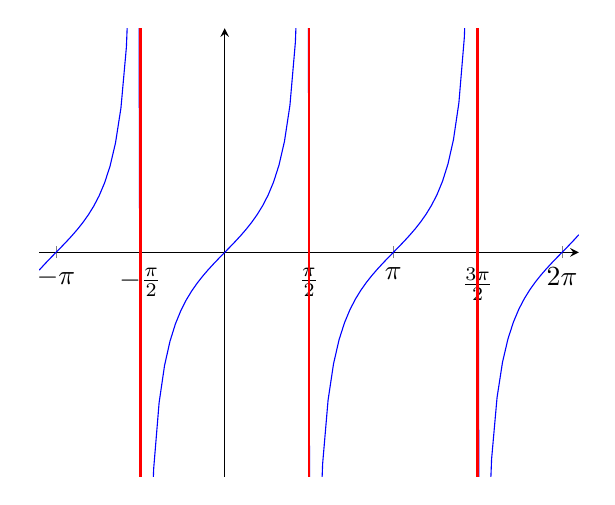
\begin{tikzpicture}
\begin{axis}[
  axis x line=center, axis y line=center,
  ymax=4.1,ymin=-4.1, ymajorticks=false,
  xtick={-3.141592654,-1.570796327,1.570796327,3.141592654,4.71238898,6.283185307},
  xticklabels={$-\pi$, $-\frac{\pi}{2}$, $\frac{\pi}{2}$, $\pi$, $\frac{3\pi}{2}$,$2\pi$}
  ]
\addplot[blue,domain=-1.1*pi:2.1*pi,samples=100] {tan(deg(x))};

\addplot[line width=1pt,red] coordinates {(-1.570796327,4.15) (-1.570796327,-4.15)};
\addplot[line width=1pt,red] coordinates {(1.570796327,4.15) (1.570796327,-4.15)};
\addplot[line width=1pt,red] coordinates {(4.71238898,4.15) (4.71238898,-4.15)};
\end{axis}
\end{tikzpicture}
\end{tabular}
\end{center}

\section{Trigonometry --- Special Triangles}
\begin{center}
  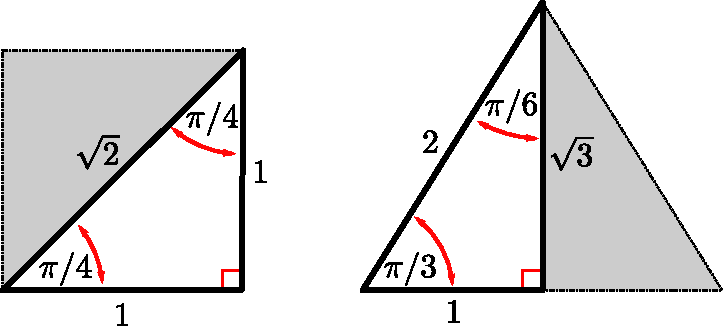
\includegraphics[height=4cm]{special_triangles}
\end{center}
From the above pair of special triangles we have
\begin{align*}
  \sin \frac{\pi}{4} &= \frac{1}{\sqrt{2}} &  \sin \frac{\pi}{6} &= \frac{1}{2} & \sin \frac{\pi}{3} &= \frac{\sqrt{3}}{2} \\
  \cos \frac{\pi}{4} &= \frac{1}{\sqrt{2}} &  \cos \frac{\pi}{6} &= \frac{\sqrt{3}}{2} & \cos \frac{\pi}{3} &= \frac{1}{2} \\
  \tan \frac{\pi}{4} &= 1 &  \tan \frac{\pi}{6} &= \frac{1}{\sqrt{3}} & \tan
\frac{\pi}{3} &= \sqrt{3}
\end{align*}

\section{Trigonometry --- Simple Identities}
\begin{itemize}
 \item Periodicity
\begin{align*}
  \sin(\theta+2\pi) &= \sin(\theta) &
  \cos(\theta+2\pi) &= \cos(\theta)
\end{align*}
\item Reflection
\begin{align*}
  \sin(-\theta)&=-\sin(\theta) & \cos(-\theta) &=\cos(\theta)
%   \sin(\pi-\theta)&=\sin(\theta) & \cos(\pi-\theta) &=\cos(\theta) \\
%   \sin(\pi+\theta)&=-\sin(\theta) & \cos(\pi+\theta) &=-\cos(\theta)
\end{align*}
\item Reflection around $\pi/4$
\begin{align*}
\sin\left(\tfrac{\pi}{2}-\theta\right)&=\cos\theta &
\cos\left(\tfrac{\pi}{2}-\theta\right)&=\sin\theta
\end{align*}
\item Reflection around $\pi/2$
\begin{align*}
\sin\left(\pi-\theta\right)&=\sin\theta &
\cos\left(\pi-\theta\right)&=-\cos\theta
\end{align*}
\item Rotation by $\pi$
\begin{align*}
\sin\left(\theta+\pi\right)&=-\sin\theta &
\cos\left(\theta+\pi\right)&=-\cos\theta
\end{align*}
\item Pythagoras
\begin{align*}
\sin^2\theta + \cos^2 \theta &=1
\end{align*}

\end{itemize}

\section{Trigonometry --- Add and Subtract Angles}\label{sec trig add}
\begin{itemize}
 \item Sine
\begin{align*}
  \sin(\alpha \pm \beta) &= \sin(\alpha)\cos(\beta) \pm \cos(\alpha)\sin(\beta)
  \end{align*}
 \item Cosine
\begin{align*}
  \cos(\alpha \pm \beta) &= \cos(\alpha)\cos(\beta) \mp \sin(\alpha)\sin(\beta)
\end{align*}

\end{itemize}

\section{Inverse Trigonometric Functions}\label{sec inv trig}
Some of you may not have studied inverse trigonometric functions in highschool, however
we still expect you to know them by the end of the course.
\begin{center}
\renewcommand{\arraystretch}{1.5}
\begin{tabular}{|c|c|c|}
\hline
$\arcsin x$ & $\arccos x$ & $\arctan x$\\
\hline
Domain: $-1 \leq x \leq 1$&
Domain: $-1 \leq x \leq 1$&
Domain: all real numbers\\
Range: $-\frac{\pi}{2} \leq \arcsin x \leq \frac{\pi}{2}$&
Range: $0 \leq \arccos x \leq \pi$&
Range: $-\frac{\pi}{2} < \arctan x < \frac{\pi}{2}$\\
\hline
\begin{tikzpicture} 
\begin{axis}[
  legend pos = north west,
  axis x line=center, axis y line=center, 
  xmax=1.1,xmin=-1.1, xtick={-1,1},
  ymin=-2, ymax=2,
  ytick={-1.570796327,1.570796327},
  yticklabels={$-\nicefrac{\pi}{2}$, $\nicefrac{\pi}{2}$}
  ]
\addplot[blue, line width=1pt, domain=-1:1,samples=100] {asin(x)/180*pi}; 
% \legend{$\arcsin \theta$}
\end{axis}
\end{tikzpicture}
&
\begin{tikzpicture} 
\useasboundingbox (0,0) rectangle (5,4.2);
\begin{axis}[
  axis x line=center, axis y line=center, 
  xmax=1.1,xmin=-1.1, xtick={-1,1},
  ymin=-0.3,ymax=3.4,
  ytick={0,1.570796327,3.141592654},
  yticklabels={0,$\nicefrac{\pi}{2}$, $\pi$}
  ]
 \addplot[blue, line width=1pt, domain=-1:1,samples=100] {acos(x)/180*pi}; 
% \legend{$\cos \theta$}
\end{axis}
\end{tikzpicture}
&
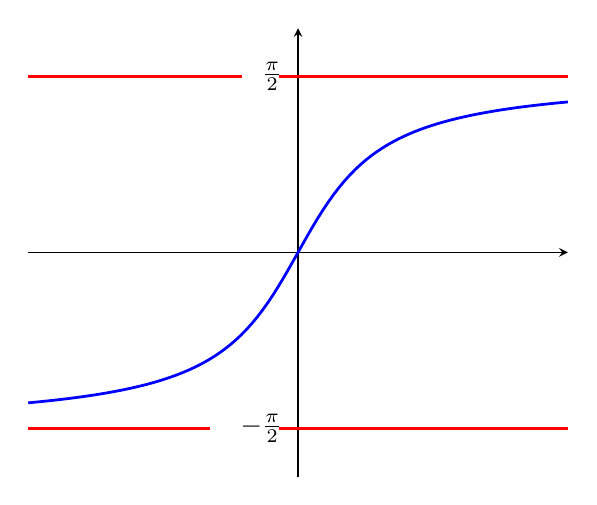
\begin{tikzpicture} 
\begin{axis}[
  legend pos = north west,
  axis x line=center, axis y line=center, 
  xmax=4.3,xmin=-4.3, xmajorticks=false,
  ymin=-2,ymax=2,
  ytick={-1.570796327,1.570796327},
  yticklabels={$-\frac{\pi}{2}$, $\frac{\pi}{2}$}
  ]
\addplot[blue, line width=1pt, domain=-4.3:4.3,samples=100] {atan(x)/180*pi}; 
% \legend{$\tan \theta$}

\addplot[line width=1pt,red] coordinates {(4.3,-1.570796327) (-0.3,-1.570796327)};
\addplot[line width=1pt,red] coordinates {(-1.4,-1.570796327) (-4.3,-1.570796327)};
\addplot[line width=1pt,red] coordinates {(4.3,1.570796327) (-0.3,1.570796327)};
\addplot[line width=1pt,red] coordinates {(-0.9,1.570796327) (-4.3,1.570796327)};
\end{axis}
\end{tikzpicture}
\\ \hline
\end{tabular}
\renewcommand{\arraystretch}{1}
\end{center}
Since these functions are inverses of each other we have
\begin{align*}
  \arcsin(\sin \theta) &= \theta & -\frac{\pi}{2} \leq \theta \leq \frac{\pi}{2} \\
  \arccos(\cos \theta) &= \theta & 0 \leq \theta \leq \pi \\
  \arctan(\tan \theta) &= \theta & -\frac{\pi}{2} \leq \theta \leq \frac{\pi}{2}	
\end{align*}
and also
\begin{align*}
  \sin(\arcsin x) &= x & -1 \leq x \leq 1 \\
  \cos(\arccos x) &= x & -1 \leq x \leq 1 \\
  \tan(\arctan x) &= x & \text{any real $x$}
\end{align*}
%The compositions of trignometric and inverse trigonometric functions are
%\begin{align*}
%  \sin( \arcsin x ) &= x & 
%  \sin( \arccos x ) &= \sqrt{1-x^2} & 
%  \sin( \arctan x ) &= \frac{x}{\sqrt{1+x^2}} \\ 
%%
%  \cos( \arcsin x ) &= \sqrt{1-x^2} & 
%  \cos( \arccos x ) &= x &
%  \cos( \arctan x ) &= \frac{1}{\sqrt{1+x^2}} \\ 
%%
%  \tan( \arcsin x ) &= \frac{x}{\sqrt{1-x^2}} & 
%  \tan( \arccos x ) &= \frac{\sqrt{1-x^2}}{x} &
%  \tan( \arctan x ) &= x 
%\end{align*}

\begin{center}
\renewcommand{\arraystretch}{1.5}
\begin{tabular}{|c|c|c|}
\hline
$\arccsc x$ & $\arcsec x$ & $\arccot x$\\
\hline
Domain: $|x|\ge 1$&
Domain: $|x|\ge 1$&
Domain: all real numbers\\
Range: $-\frac{\pi}{2} \leq \arccsc x \leq \frac{\pi}{2}$&
Range: $0 \leq \arcsec x \leq \pi$&
Range: $0 < \arccot x < \pi$\\[-0.1in]
       $\arccsc x \ne 0$ &
       $\arcsec x \ne \frac{\pi}{2}$ &
        \\
\hline
\begin{tikzpicture} 
\begin{axis}[
  legend pos = north west,
  axis x line=center, axis y line=center, 
  xmax=4.3,xmin=-4.3, xtick={-1,1},
  ymin=-2, ymax=2,
  ytick={-1.570796327,1.570796327},
  yticklabels={$-\frac{\pi}{2}\!\!\!$, $\frac{\pi}{2}$}
  ]
\addplot[blue, line width=1pt, domain=1:4.3,samples=50] {asin(1/x)/180*pi}; 
\addplot[blue, line width=1pt, domain=-4.3:-1,samples=50] {asin(1/x)/180*pi}; 
\end{axis}
\end{tikzpicture}
&
\begin{tikzpicture} 
\useasboundingbox (0,0) rectangle (5,4.2);
\begin{axis}[
  axis x line=center, axis y line=center, 
  xmax=4.3,xmin=-4.3, xtick={-1,1},
  ymin=-0.3,ymax=3.4,
  ytick={0,1.570796327,3.141592654},
  yticklabels={0,$\frac{\pi}{2}$, $\pi$}
  ]
 \addplot[blue, line width=1pt, domain=1:4.3,samples=100] {acos(1/x)/180*pi}; 
 \addplot[blue, line width=1pt, domain=-4.3:-1,samples=100] {acos(1/x)/180*pi}; 
% \legend{$\cos \theta$}
\end{axis}
\end{tikzpicture}
&
\begin{tikzpicture} 
\begin{axis}[
  legend pos = north west,
  axis x line=center, axis y line=center, 
  xmax=4.3,xmin=-4.3, xmajorticks=false,
  ymin=-0.3,ymax=3.4,
  ytick={0,1.570796327,3.141592654},
  yticklabels={0,$\frac{\pi}{2}$, $\pi$}
  ]
\addplot[blue, line width=1pt, domain=-4.3:-0.01,samples=100] {atan(1/x)/180*pi + pi}; 
\addplot[blue, line width=1pt, domain=0.01:4.3,samples=100] {atan(1/x)/180*pi}; 
% \legend{$\tan \theta$}

\addplot[line width=1pt,red] coordinates {(4.3,3.141592654) (-0.3,3.141592654)};
\addplot[line width=1pt,red] coordinates {(-0.9,3.141592654) (-4.3,3.141592654)};
\end{axis}
\end{tikzpicture}
\\ \hline
\end{tabular}
\renewcommand{\arraystretch}{1}
\end{center}
Again
\begin{align*}
  \arccsc(\csc \theta) &= \theta & -\frac{\pi}{2} \leq \theta \leq \frac{\pi}{2},\ \theta\ne 0 \\
  \arcsec(\sec \theta) &= \theta & 0 \leq \theta \leq \pi,\ \theta\ne \frac{\pi}{2} \\
  \arccot(\cot \theta) &= \theta & 0 < \theta < \pi	
\end{align*}
and 
\begin{align*}
  \csc(\arccsc x) &= x & |x|\ge 1 \\
  \sec(\arcsec x) &= x & |x|\ge 1 \\
  \cot(\arccot x) &= x & \text{any real $x$}
\end{align*}

\section{Areas}\label{app sec areas}
\begin{center}
 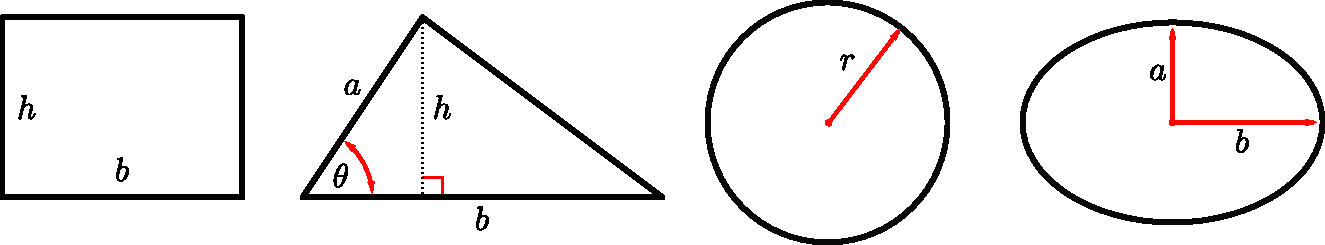
\includegraphics[width=\textwidth]{area2d}
\end{center}
\begin{itemize}
 \item Area of a rectangle
\begin{align*}
  A &= b h
\end{align*}
 \item Area of a triangle
\begin{align*}
  A &= \frac{1}{2} b h = \frac{1}{2} ab \sin \theta
\end{align*}
 \item Area of a circle
\begin{align*}
  A &= \pi r^2
\end{align*}
 \item Area of an ellipse
\begin{align*}
  A &= \pi ab
\end{align*}
\end{itemize}

\section{Volumes}\label{sec volumes}
\begin{center}
 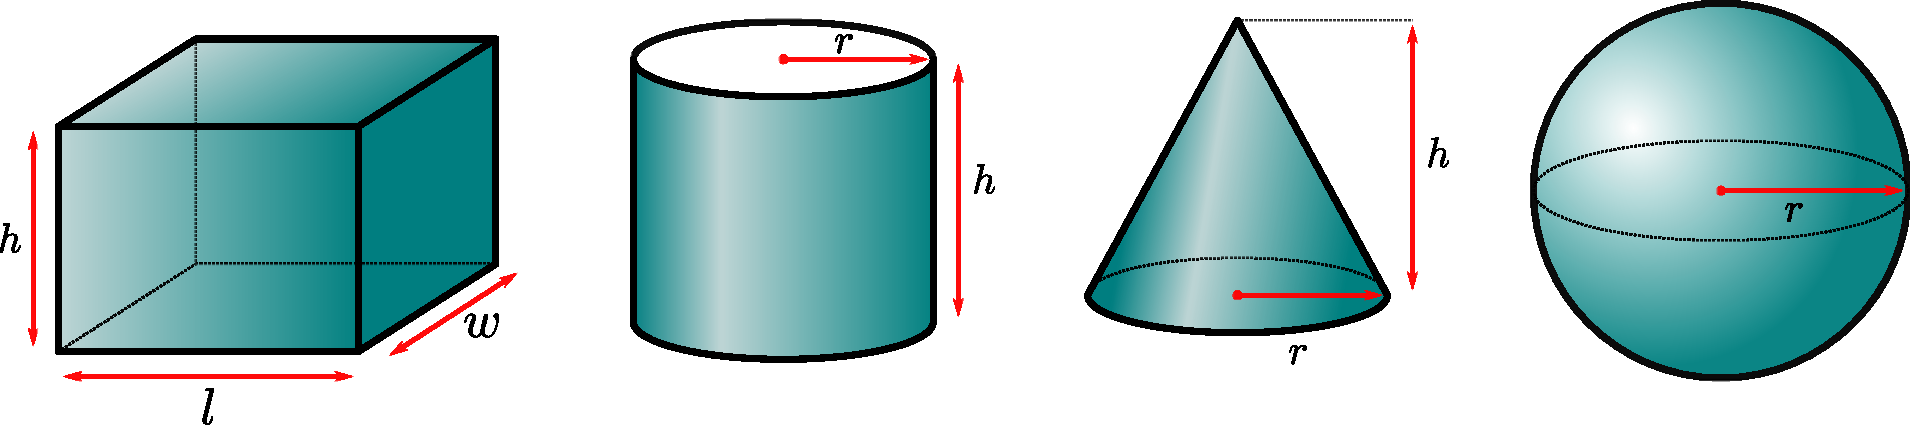
\includegraphics[width=\textwidth]{vol3d}
\end{center}
\begin{itemize}
 \item Volume of a rectangular prism
\begin{align*}
  V &= l w h
\end{align*}
 \item Volume of a cylinder
\begin{align*}
  V &= \pi r^2 h
\end{align*}
 \item Volume of a cone
\begin{align*}
  V &= \frac{1}{3} \pi r^2 h
\end{align*}

 \item Volume of a sphere
\begin{align*}
  V &= \frac{4}{3} \pi r^3
\end{align*}
\end{itemize}


\section{Powers}\label{sec powers}
In the following, $x$ and $y$ are arbitrary real numbers,
and $q$ is an arbitrary constant that is strictly bigger
than zero.
\begin{itemize}
 \item $q^0=1$

\item $q^{x+y}=q^xq^y$,
         $q^{x-y}=\frac{q^x}{q^y}$
\item $q^{-x}=\frac{1}{q^x}$
\item $\big(q^x\big)^y=q^{xy}$
\item  $\lim\limits_{x\rightarrow\infty}q^x=\infty$,
           $\lim\limits_{x\rightarrow-\infty}q^x=0$ if $q>1$
\item $\lim\limits_{x\rightarrow\infty}q^x=0$,
           $\lim\limits_{x\rightarrow-\infty}q^x=\infty$ if $0<q<1$
\item  The graph of $2^x$ is given below. The graph of  $q^x$,
for any $q>1$, is similar.

\begin{center}
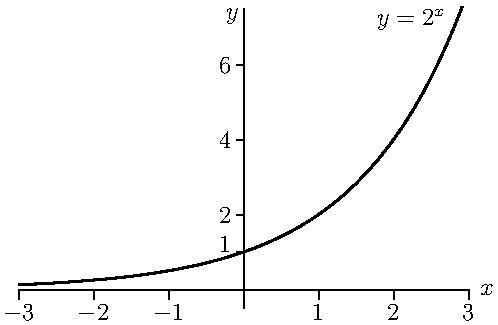
\includegraphics{expGraph2}
\end{center}


\end{itemize}


\section{Logarithms}\label{sec logs}

In the following, $x$ and $y$ are arbitrary real numbers that
are strictly bigger than 0, and
$p$ and $q$ are arbitrary constants that are strictly bigger than one.

\begin{itemize}
\item   $q^{\log_q x}=x$,\ \ \
            $\log_q \big(q^x\big)=x$
\item   $\log_q x=\frac{\log_p x}{\log_p q}$
\item  $\log_q 1=0$,\ \ \
          $\log_q q=1$
\item $\log_q(xy)=\log_q x+\log_q y$
\item $\log_q\big(\frac{x}{y}\big)=\log_q x-\log_q y$
\item $\log_q\big(\frac{1}{y}\big)=-\log_q y$,
\item $\log_q(x^y)=y\log_q x$
\item $\lim\limits_{x\rightarrow\infty}\log_q x=\infty$, \ \ \
           $\lim\limits_{x\rightarrow0}\log_q x=-\infty$
\item The graph of $\log_{10} x$ is given below. The graph of  $\log_q x$,
for any $q>1$, is similar.

\begin{center}
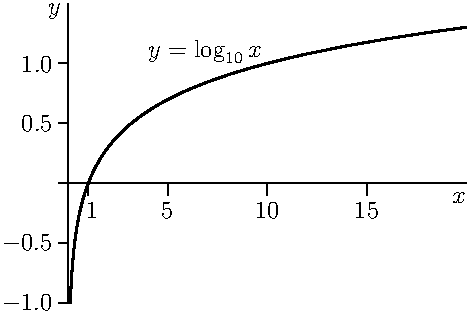
\includegraphics{logGraph10}
\end{center}

\end{itemize}



\longsection{Highschool Material You Should be Able to Derive}{You should be
able to derive}
\label{sec must deriv}
\begin{itemize}
 \item Graphs of $\csc\theta, \sec \theta$ and $\cot \theta$:
\end{itemize}
\begin{center}
\begin{tabular}{ccc}
$\csc \theta$ & $\sec \theta$ & $\cot \theta$ \\
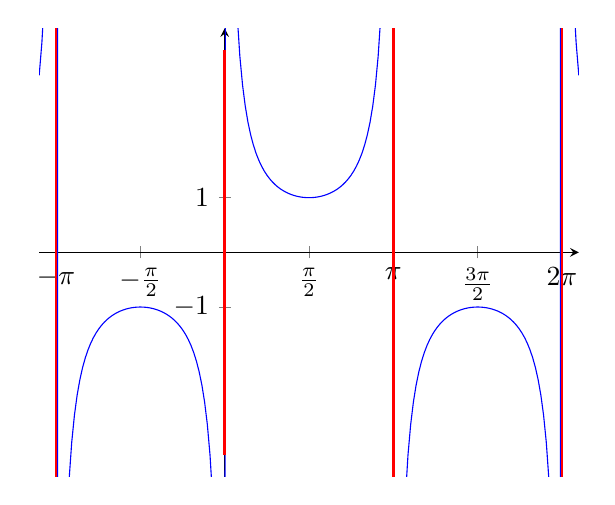
\begin{tikzpicture}
\begin{axis}[
  axis x line=center, axis y line=center,
  ymax=4.1,ymin=-4.1,ytick={-1,1},
  xtick={-3.141592654,-1.570796327,1.570796327,3.141592654,4.71238898,6.283185307},
  xticklabels={$-\pi$, $-\frac{\pi}{2}$, $\frac{\pi}{2}$, $\pi$, $\frac{3\pi}{2}$,$2\pi$}
  ]
\addplot[blue,domain=-1.1*pi:2.1*pi,samples=200] {cosec(deg(x))};
% \legend{$\csc \theta$}

\addplot[line width=1pt,red] coordinates {(-3.141592654,4.15) (-3.141592654,-4.15)};
\addplot[line width=1pt,red] coordinates {(0,3.7) (0,-3.7)};
\addplot[line width=1pt,red] coordinates {(3.141592654,4.15) (3.141592654,-4.15)};
\addplot[line width=1pt,red] coordinates {(6.283185307,4.15) (6.283185307,-4.15)};
\end{axis}
\end{tikzpicture}
&
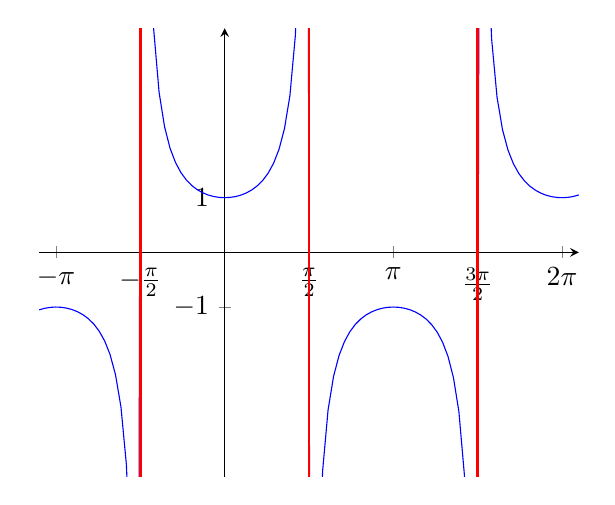
\begin{tikzpicture}
\begin{axis}[
  axis x line=center, axis y line=center,
  ymax=4.1,ymin=-4.1, ytick={-1,1},
  xtick={-3.141592654,-1.570796327,1.570796327,3.141592654,4.71238898,6.283185307},
  xticklabels={$-\pi$, $-\frac{\pi}{2}$, $\frac{\pi}{2}$, $\pi$, $\frac{3\pi}{2}$,$2\pi$}
  ]
\addplot[blue,domain=-1.1*pi:2.1*pi,samples=100] {sec(deg(x))};
% \legend{$\sec \theta$}
\addplot[line width=1pt,red] coordinates {(-1.570796327,4.15) (-1.570796327,-4.15)};
\addplot[line width=1pt,red] coordinates {(1.570796327,4.15) (1.570796327,-4.15)};
\addplot[line width=1pt,red] coordinates {(4.71238898,4.15) (4.71238898,-4.15)};

\end{axis}
\end{tikzpicture}
&
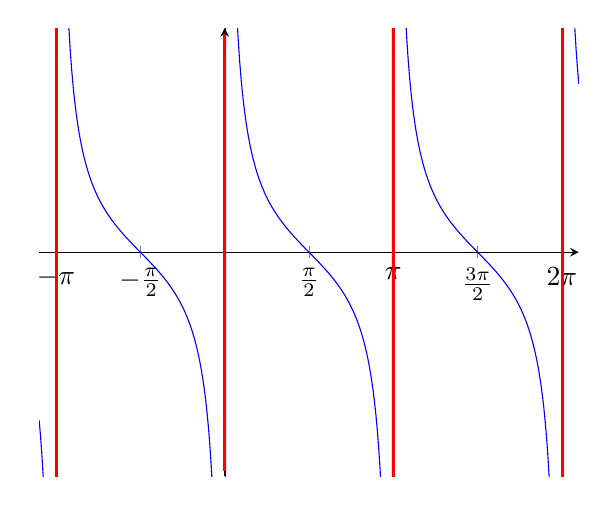
\begin{tikzpicture}
\begin{axis}[
  axis x line=center, axis y line=center,
  ymax=4.1,ymin=-4.1, ymajorticks=false,
  xtick={-3.141592654,-1.570796327,1.570796327,3.141592654,4.71238898,6.283185307},
  xticklabels={$-\pi$, $-\frac{\pi}{2}$, $\frac{\pi}{2}$, $\pi$, $\frac{3\pi}{2}$,$2\pi$}
  ]
\addplot[blue,domain=-1.1*pi:2.1*pi,samples=400] {cot(deg(x))};
% \legend{$\cot \theta$}

\addplot[line width=1pt,red] coordinates {(-3.14,4.15) (-3.14,-4.15)};
\addplot[line width=1pt,red] coordinates {(0,4) (0,-4)};
\addplot[line width=1pt,red] coordinates {(3.14,4.15) (3.14,-4.15)};
\addplot[line width=1pt,red] coordinates {(6.3,4.15) (6.3,-4.15)};
\end{axis}
\end{tikzpicture}
\end{tabular}
\end{center}
\begin{itemize}
 \item More Pythagoras
\begin{align*}
\sin^2\theta + \cos^2 \theta &=1 & \xmapsto{\text{divide by $\cos^2\theta$}}&&
\tan^2\theta + 1  &= \sec^2\theta \\
\sin^2\theta + \cos^2 \theta &=1 & \xmapsto{\text{divide by $\sin^2\theta$}}&&
1 + \cot^2 \theta &=\csc^2\theta
\end{align*}

 \item Sine --- double angle (set $\beta =\alpha$ in sine angle addition formula)
\begin{align*}
  \sin(2\alpha) &= 2\sin(\alpha)\cos(\alpha)
\end{align*}
 \item Cosine --- double angle (set $\beta =\alpha$ in cosine angle addition formula)
\begin{align*}
  \cos(2\alpha) &= \cos^2(\alpha) - \sin^2(\alpha) \\
  &= 2\cos^2(\alpha) - 1  & \text{(use $\sin^2(\alpha)= 1-\cos^2(\alpha)$)}\\
  &= 1 - 2\sin^2(\alpha) & \text{(use $\cos^2(\alpha)= 1-\sin^2(\alpha)$)}
\end{align*}
% \item Tangent --- double angle (use the two previous double-angle identities)
% \begin{align*}
%   \tan( 2 \alpha) &= \frac{2\sin(\alpha)\cos(\alpha)}{\cos^2(\alpha) - \sin^2(\alpha)}
%   & \text{now divide numerator and denominator by $\cos^2(\alpha)$}\\
%   &= \frac{2 \tan(\alpha) }{1 - \tan^2(\alpha)}
% \end{align*}
\item Composition of trigonometric and inverse trigonometric functions:
\begin{align*}
  \cos( \arcsin x) &= \sqrt{1-x^2} &
  \sec( \arctan x) &= \sqrt{1+x^2}
\end{align*}
and similar expressions.
\end{itemize}


\begin{comment}
\chapter{Origin of Trig, Area and Volume Formulas}
\section{Theorems about Triangles}
\subsection{Thales' Theorem}
We want to get at right-angled triangles. A classic construction for this is to
draw a triangle inside a circle, so that all three corners lie on the circle
and the longest side forms the diameter of the circle. See the figure below in
which we have scaled the circle to have radius 1 and the triangle has longest
side 2.

\begin{center}
  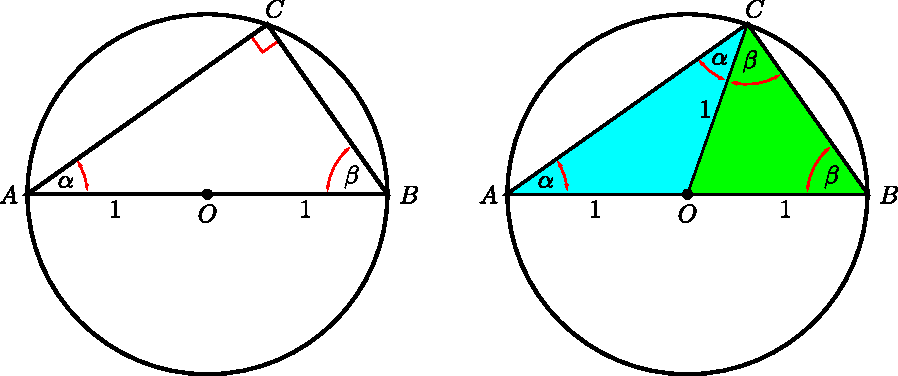
\includegraphics[height=4cm]{thales}
\end{center}

Thales theorem states that the angle at $C$ is always a right-angle. The proof
is quite straight-forward and relies on two facts:
\begin{itemize}
 \item the angles of a triangle add to $\pi$, and
 \item the angles at the base of an isosceles triangle are equal.
\end{itemize}
So we split the triangle $ABC$ by drawing a line from the centre of the circle to $C$. This creates two isosceles triangles $OAC$ and $OBC$. Since they are isosceles, the angles at their bases $\alpha$ and $\beta$ must be equal (as shown).  Adding the angles of the original triangle now gives
\begin{align*}
  \pi &= \alpha + (\alpha+\beta) + \beta = 2(\alpha+\beta)
\end{align*}
So the angle at $C = \pi - (\alpha+\beta) = \pi/2$.


\subsection{Pythagoras}
Since trigonometry, at its core, is the study of lengths and angles in right-angled
triangles, we must include a result you all know well, but likely do not know how to
prove.
\begin{center}
  \includegraphics[height=3.5cm]{right_triangle}
\end{center}
The lengths of the sides of any right-angled triangle are related by the famous result due to Pythagoras
\begin{align*}
  c^2 &= a^2+b^2.
\end{align*}
There are many ways to prove this, but we can do so quite simply by studying the following diagram:
\begin{center}
  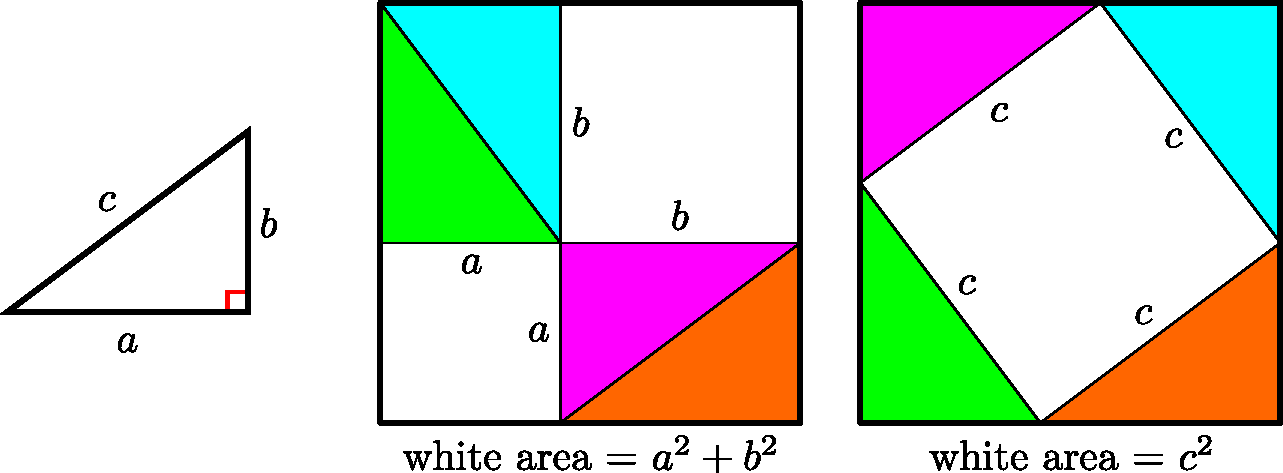
\includegraphics[height=4cm]{pythag}
\end{center}
We start with a right-angled triangle with sides labeled $a,b$ and $c$. Then we construct a square of side-length $a+b$ and draw inside it 4 copies of the triangle arranged as shown in the centre of the above figure. The area in white is then $a^2+b^2$. Now move the triangles around to create the arrangement shown on the right of the above figure. The area in white is bounded by a square of side-length $c$ and so its area is $c^2$. The area of the outer square didn't change when the triangles were moved, nor did the area of the triangles, so the white area cannot have changed either. This proves $a^2+b^2=c^2$.


\section{Trigonometry}
\subsection{Angles --- Radians vs Degrees}\label{ssec rad deg}
For mathematics, and especially in calculus, it is much better to measure angles in units
called radians rather than degrees. By definition, an arc of length $\theta$ on a circle
of radius one subtends an angle of $\theta$ radians at the centre of the
circle.
\begin{center}
 \includegraphics[height=4cm]{radian}
\end{center}
The circle on the left has radius 1, and the arc swept out by an angle of
$\theta$ radians has length~$\theta$. Because a circle of radius one has circumference
$2\pi$ we have
\begin{align*}
   2\pi\text{ radians }&=360^\circ &
    \pi\text{ radians }&=180^\circ &
    \nicefrac{\pi}{2}\text{ radians }&=90^\circ \\
%%
  \frac{\pi}{3}\text{ radians }&=60^\circ &
  \frac{\pi}{4}\text{ radians }&=45^\circ &
  \frac{\pi}{6}\text{ radians }&=30^\circ
\end{align*}

More generally, consider a circle of radius $r$. Let $L(\theta)$ denote the length of
the arc swept out by an angle of $\theta$ radians and let $A(\theta)$ denote the area of
the sector (or wedge) swept out by the same angle. Since the angle sweeps out the
fraction $\nicefrac{\theta}{2\pi}$ of a whole circle, we have
\begin{align*}
  L(\theta) &= 2\pi r \cdot \frac{\theta}{2\pi} = \theta r & \text{and}\\
  A(\theta) &= \pi r^2 \cdot \frac{\theta}{2\pi} = \frac{\theta}{2} r^2
\end{align*}

\subsection{Trig Function Definitions}
The trigonometric functions are defined as ratios of the lengths of the sides of a
right-angle triangle as shown in the left of the diagram below . These ratios depend only
on the angle~$\theta$.
\begin{center}
  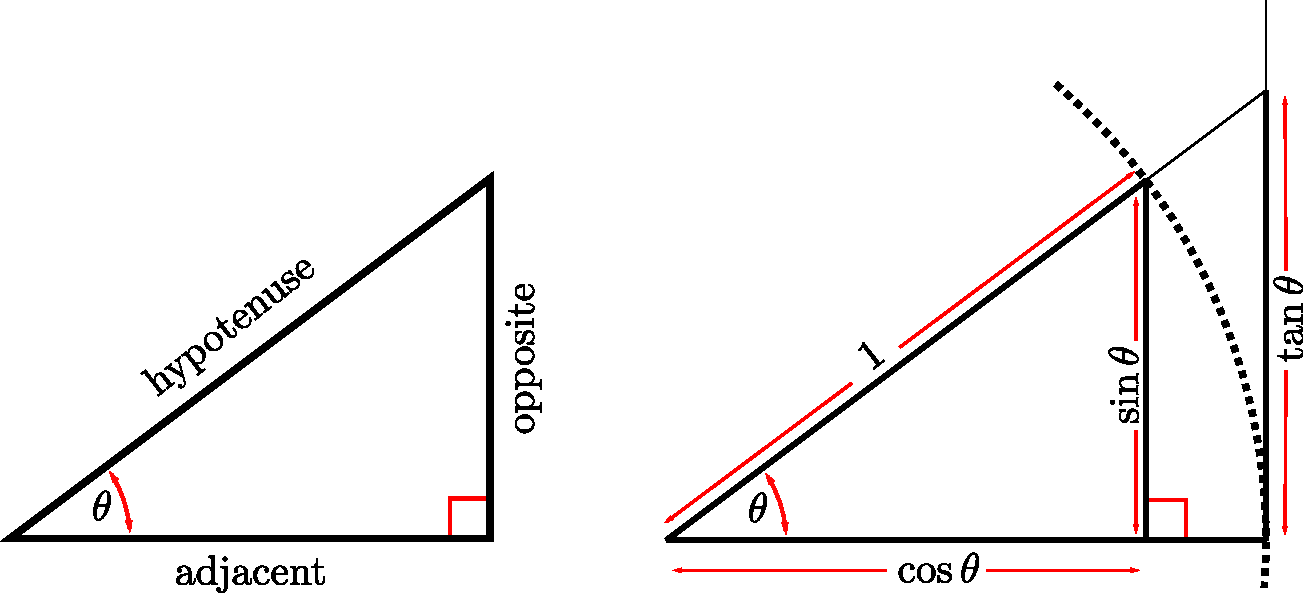
\includegraphics[height=5cm]{trig_defn}
\end{center}
The trigonometric functions sine, cosine and tangent are defined as ratios of
the lengths of the sides
\begin{align*}
% \text{sine} && \text{cosine} && \text{tangent}\\
\sin\theta &= \frac{\text{opposite}}{\text{hypotenuse}} &
\cos\theta &= \frac{\text{adjacent}}{\text{hypotenuse}} &
\tan\theta &= \frac{\text{opposite}}{\text{adjacent}} = \frac{\sin \theta}{\cos \theta}.
\intertext{These are frequently abbreviated as}
\sin\theta &= \frac{\text{o}}{\text{h}} &
\cos\theta &= \frac{\text{a}}{\text{h}} &
\tan\theta &= \frac{\text{o}}{\text{a}}
\end{align*}
which gives rise to the mnemonic
\begin{align*}
  \text{SOH} && \text{CAH} && \text{TOA}
\end{align*}
If we scale the triangle so that they hypotenuse has length $1$ then we obtain the
diagram on the right. In that case, $\sin \theta$ is the height of the triangle, $\cos
\theta$ the length of its base and $\tan \theta$ is the length of the line tangent to the
circle of radius 1 as shown.

Since the angle $2\pi$ sweeps out a full circle, the angles $\theta$ and $\theta+2\pi$
are really the same.
\begin{center}
  \includegraphics[height=5cm]{trig_defn3}
\end{center}
Hence all the trigonometric functions are periodic with period $2\pi$. That is
\begin{align*}
  \sin(\theta+2\pi) &= \sin(\theta) &
  \cos(\theta+2\pi) &= \cos(\theta) &
  \tan(\theta+2\pi) &= \tan(\theta)
\end{align*}
The plots of these functions are shown below
\begin{center}
\begin{tabular}{ccc}
$\sin \theta$ & $\cos \theta$ & $\tan \theta$
\\
\begin{tikzpicture}
\begin{axis}[
  axis x line=center, axis y line=center,
  ymax=1.1,ymin=-1.1, ytick={-1,1},
  xtick={-3.141592654,-1.570796327,1.570796327,3.141592654,4.71238898,6.283185307},
  xticklabels={$-\pi$, $-\frac{\pi}{2}$, $\frac{\pi}{2}$, $\pi$, $\frac{3\pi}{2}$,$2\pi$}
  ]
\addplot[blue,domain=-1.1*pi:2.1*pi,samples=100] {sin(deg(x))};
\end{axis}
\end{tikzpicture}
&
\begin{tikzpicture}
\begin{axis}[
  axis x line=center, axis y line=center,
  ymax=1.1,ymin=-1.1, ytick={-1,1},
  xtick={-3.141592654,-1.570796327,1.570796327,3.141592654,4.71238898,6.283185307},
  xticklabels={$-\pi$, $-\frac{\pi}{2}$, $\frac{\pi}{2}$, $\pi$, $\frac{3\pi}{2}$,$2\pi$}
  ]
\addplot[blue,domain=-1.1*pi:2.1*pi,samples=100] {cos(deg(x))};
\end{axis}
\end{tikzpicture}
&
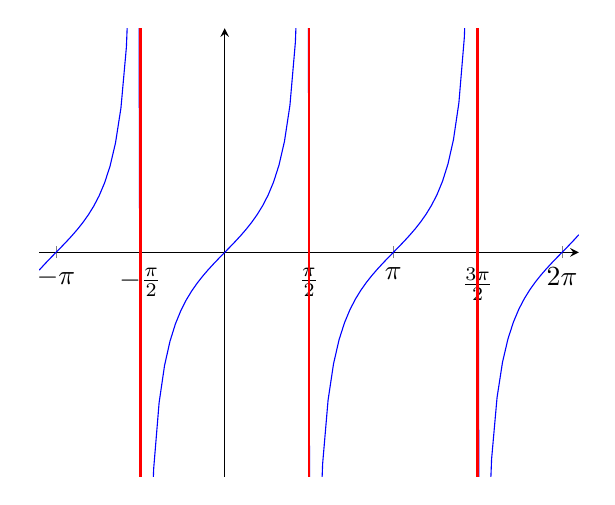
\begin{tikzpicture}
\begin{axis}[
  axis x line=center, axis y line=center,
  ymax=4.1,ymin=-4.1, ymajorticks=false,
  xtick={-3.141592654,-1.570796327,1.570796327,3.141592654,4.71238898,6.283185307},
  xticklabels={$-\pi$, $-\frac{\pi}{2}$, $\frac{\pi}{2}$, $\pi$, $\frac{3\pi}{2}$,$2\pi$}
  ]
\addplot[blue,domain=-1.1*pi:2.1*pi,samples=100] {tan(deg(x))};

\addplot[line width=1pt,red] coordinates {(-1.570796327,4.15) (-1.570796327,-4.15)};
\addplot[line width=1pt,red] coordinates {(1.570796327,4.15) (1.570796327,-4.15)};
\addplot[line width=1pt,red] coordinates {(4.71238898,4.15) (4.71238898,-4.15)};
\end{axis}
\end{tikzpicture}
\end{tabular}
\end{center}


The reciprocals (cosecant, secant and cotangent) of these functions also play important
roles in trigonometry and calculus:
\begin{align*}
% \text{cosecant} && \text{secant} && \text{cotangent}\\
\csc \theta &= \frac{1}{\sin\theta} = \frac{\text{h}}{\text{o}} &
\sec\theta &= \frac{1}{\cos \theta} = \frac{\text{h}}{\text{a}} &
\cot\theta &= \frac{1}{\tan \theta} = \frac{\cos \theta}{\sin\theta} =
\frac{\text{a}}{\text{o}}
\end{align*}
The plots of these functions are shown below
\begin{center}
\begin{tabular}{ccc}
$\csc \theta$ & $\sec \theta$ & $\cot \theta$ \\
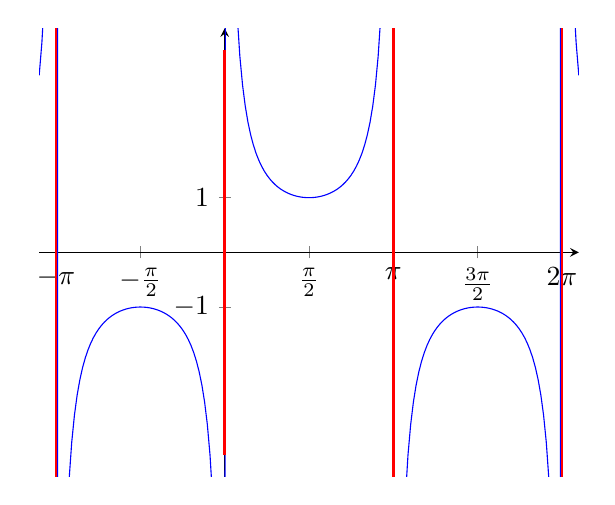
\begin{tikzpicture}
\begin{axis}[
  axis x line=center, axis y line=center,
  ymax=4.1,ymin=-4.1,ytick={-1,1},
  xtick={-3.141592654,-1.570796327,1.570796327,3.141592654,4.71238898,6.283185307},
  xticklabels={$-\pi$, $-\frac{\pi}{2}$, $\frac{\pi}{2}$, $\pi$, $\frac{3\pi}{2}$,$2\pi$}
  ]
\addplot[blue,domain=-1.1*pi:2.1*pi,samples=200] {cosec(deg(x))};
% \legend{$\csc \theta$}

\addplot[line width=1pt,red] coordinates {(-3.141592654,4.15) (-3.141592654,-4.15)};
\addplot[line width=1pt,red] coordinates {(0,3.7) (0,-3.7)};
\addplot[line width=1pt,red] coordinates {(3.141592654,4.15) (3.141592654,-4.15)};
\addplot[line width=1pt,red] coordinates {(6.283185307,4.15) (6.283185307,-4.15)};
\end{axis}
\end{tikzpicture}
&
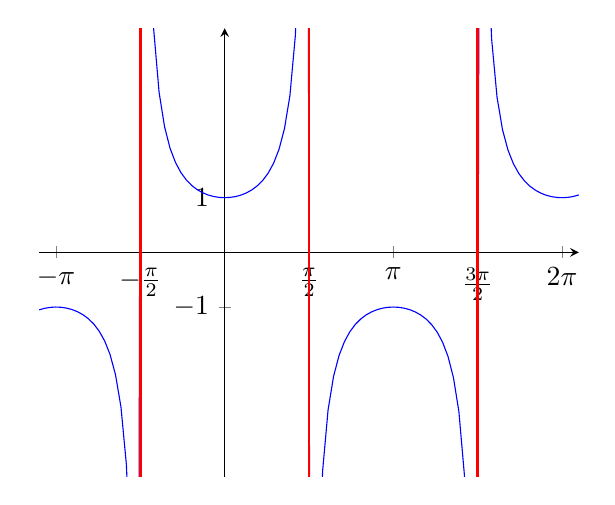
\begin{tikzpicture}
\begin{axis}[
  axis x line=center, axis y line=center,
  ymax=4.1,ymin=-4.1, ytick={-1,1},
  xtick={-3.141592654,-1.570796327,1.570796327,3.141592654,4.71238898,6.283185307},
  xticklabels={$-\pi$, $-\frac{\pi}{2}$, $\frac{\pi}{2}$, $\pi$, $\frac{3\pi}{2}$,$2\pi$}
  ]
\addplot[blue,domain=-1.1*pi:2.1*pi,samples=100] {sec(deg(x))};
% \legend{$\sec \theta$}
\addplot[line width=1pt,red] coordinates {(-1.570796327,4.15) (-1.570796327,-4.15)};
\addplot[line width=1pt,red] coordinates {(1.570796327,4.15) (1.570796327,-4.15)};
\addplot[line width=1pt,red] coordinates {(4.71238898,4.15) (4.71238898,-4.15)};

\end{axis}
\end{tikzpicture}
&
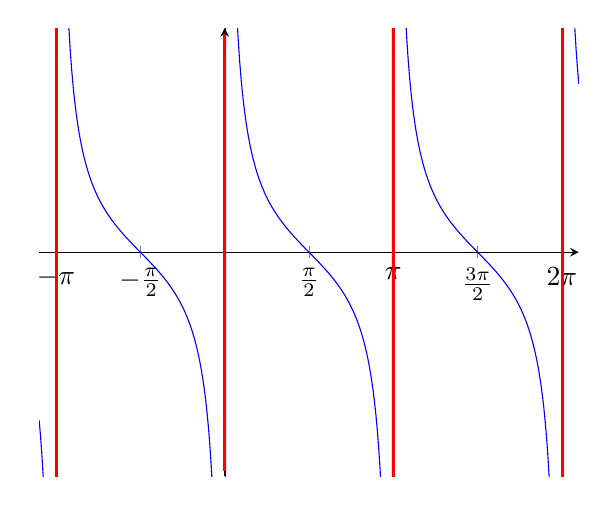
\begin{tikzpicture}
\begin{axis}[
  axis x line=center, axis y line=center,
  ymax=4.1,ymin=-4.1, ymajorticks=false,
  xtick={-3.141592654,-1.570796327,1.570796327,3.141592654,4.71238898,6.283185307},
  xticklabels={$-\pi$, $-\frac{\pi}{2}$, $\frac{\pi}{2}$, $\pi$, $\frac{3\pi}{2}$,$2\pi$}
  ]
\addplot[blue,domain=-1.1*pi:2.1*pi,samples=400] {cot(deg(x))};
% \legend{$\cot \theta$}

\addplot[line width=1pt,red] coordinates {(-3.14,4.15) (-3.14,-4.15)};
\addplot[line width=1pt,red] coordinates {(0,4) (0,-4)};
\addplot[line width=1pt,red] coordinates {(3.14,4.15) (3.14,-4.15)};
\addplot[line width=1pt,red] coordinates {(6.3,4.15) (6.3,-4.15)};
\end{axis}
\end{tikzpicture}
\end{tabular}
\end{center}



These reciprocal functions also have geometric interpretations:
\begin{center}
  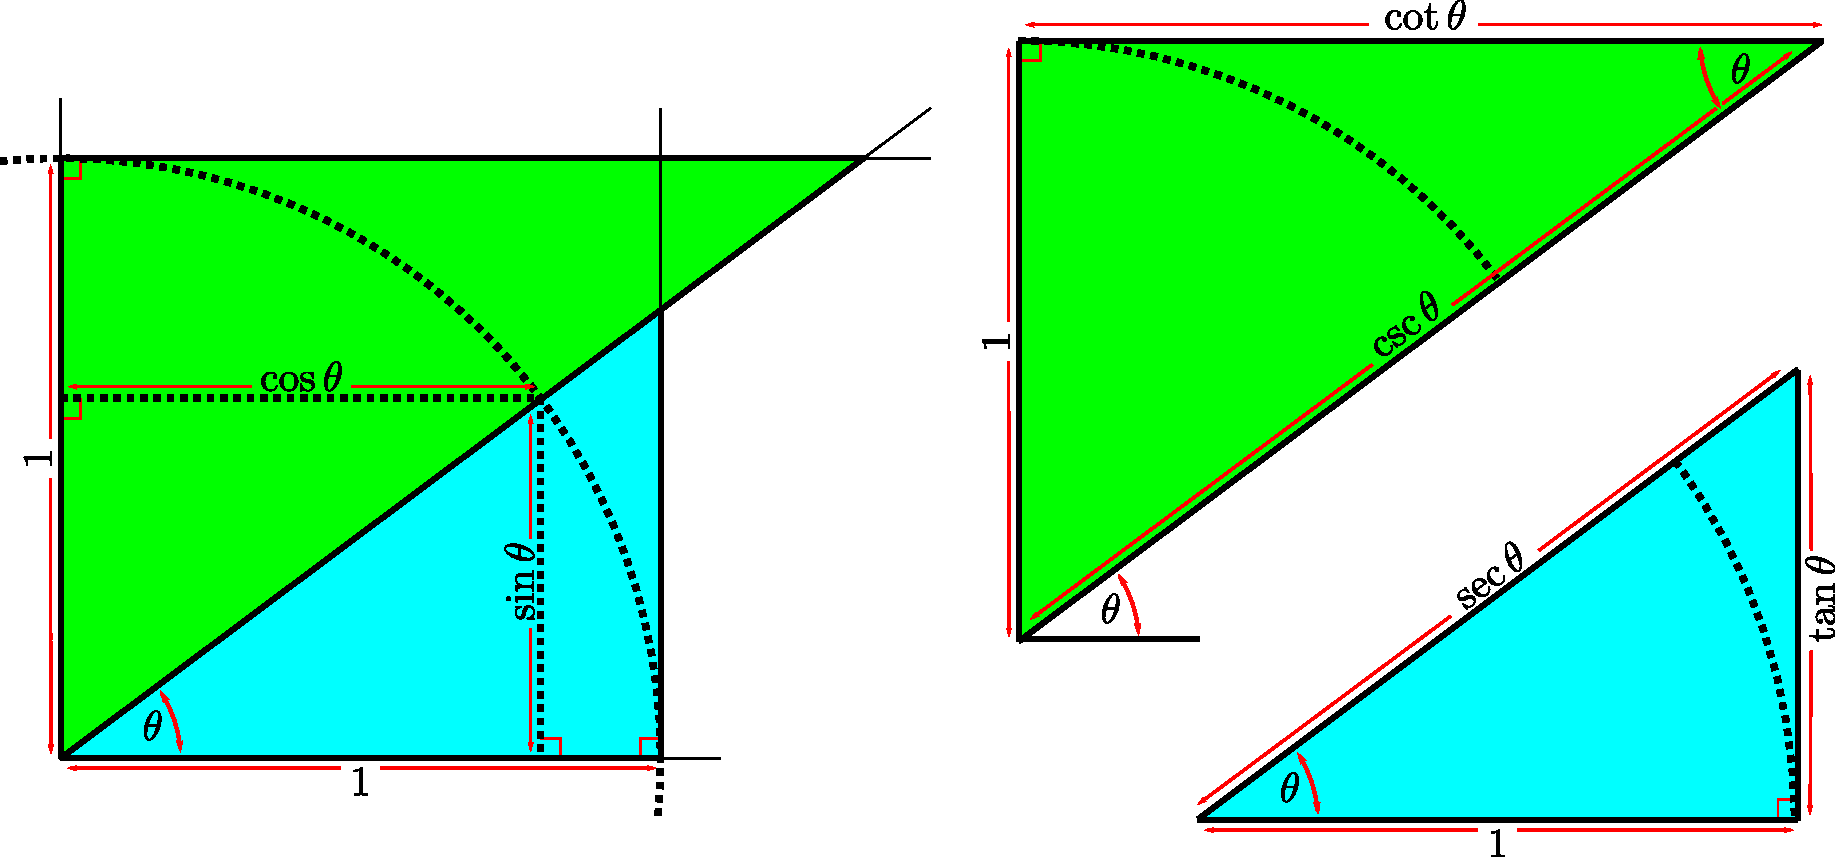
\includegraphics[height=6cm]{trig_defn2}
\end{center}
Since these are all right-angled triangles we can use Pythagoras to obtain the following
identities:
\begin{align*}
\sin^2\theta + \cos^2 \theta &=1 &
\tan^2\theta + 1  &= \sec^2\theta &
1 + \cot^2 \theta &=\csc^2\theta
\end{align*}
Of these it is only necessary to remember the first
\begin{align*}
\sin^2\theta + \cos^2 \theta &=1
\end{align*}
The second can then be obtained by dividing this by $\cos^2\theta$ and the third by
dividing by $\sin^2\theta$.


\subsection{Important Triangles}
Computing sine and cosine is non-trivial for general angles --- we need Taylor series (or
similar tools) to do this. However there are some special angles (usually small
integer fractions of $\pi$) for which we can use a little geometry to help. Consider the
following two triangles.
\begin{center}
  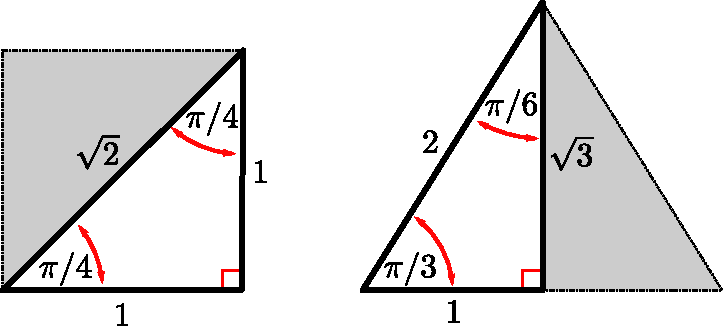
\includegraphics[height=4cm]{special_triangles}
\end{center}
The first results from cutting a square along its diagonal, while the second is obtained
by cutting an equilateral triangle from one corner to the middle of the opposite side.
These, together with the angles $0,\frac{\pi}{2}$ and $\pi$ give the following table of
values
\begin{center}
\renewcommand{\arraystretch}{1.3}
     \begin{tabular}{|c||c|c|c||c|c|c|}
          \hline
         $\theta$ & $\sin\theta$ & $\cos\theta$ & $\tan\theta$  &
                    $\csc\theta$ & $\sec\theta$ & $\cot\theta$   \\  \hline\hline
%%
        $0$ rad & 0 & 1 & 0 & DNE & 1 & DNE  \\ \hline
        $\tfrac{\pi}{2}$ rad  & 1 & 0  & DNE & 1& DNE & 0 \\ \hline
        $\pi$ rad & 0 & -1 & 0 & DNE & -1 & DNE \\ \hline\hline
%%
         $\tfrac{\pi}{4}$ rad &
            $\tfrac{1}{\sqrt{2}}$ & $\tfrac{1}{\sqrt{2}}$ & 1 &
            $\sqrt{2}$ & $\sqrt{2}$ & 1 \\ \hline\hline
%%
        $\tfrac{\pi}{6}$ rad &
            $\tfrac{1}{2}$ & $\tfrac{\sqrt{3}}{2}$ & $\tfrac{1}{\sqrt{3}}$ &
            2 & $\tfrac{2}{\sqrt{3}}$ & $\sqrt{3}$  \\ \hline
        $\tfrac{\pi}{3}$ rad &
            $\tfrac{\sqrt{3}}{2}$ & $\tfrac{1}{2}$ & $\sqrt{3}$ &
            $\tfrac{2}{\sqrt{3}}$ &  2 & $\tfrac{1}{\sqrt{3}}$  \\ \hline
     \end{tabular}
\renewcommand{\arraystretch}{1.0}
\end{center}




\subsection{Some More Simple Identities}
Consider the figure below
\begin{center}
 \includegraphics[height=55mm]{trig_defn4}
\end{center}
The pair triangles on the left shows that there is a simple relationship between
trigonometric functions evaluated at $\theta$ and at $-\theta$:
\begin{align*}
  \sin(-\theta)&=-\sin(\theta) & \cos(-\theta) &=\cos(\theta)
\end{align*}
That is --- sine is an odd function, while cosine is even. Since the other trigonometric
functions can be expressed in terms of sine and cosine we obtain
\begin{align*}
  \tan(-\theta) &=-\tan(\theta) &
  \csc(-\theta) &=-\csc(\theta) &
  \sec(-\theta) &=\sec(\theta) &
  \cot(-\theta) &=-\cot(\theta)
\end{align*}
Now consider the triangle on the right --- if we consider the angle
$\frac{\pi}{2}-\theta$ the side-lengths of the triangle remain unchanged, but the roles
of ``opposite'' and ``adjacent'' are swapped. Hence we have
\begin{align*}
\sin\left(\tfrac{\pi}{2}-\theta\right)&=\cos\theta &
\cos\left(\tfrac{\pi}{2}-\theta\right)&=\sin\theta
\end{align*}
Again these imply that
\begin{align*}
\tan\left(\tfrac{\pi}{2}-\theta\right)&=\cot\theta &
\csc\left(\tfrac{\pi}{2}-\theta\right)&=\sec\theta &
\sec\left(\tfrac{\pi}{2}-\theta\right)&=\csc\theta &
\cot\left(\tfrac{\pi}{2}-\theta\right)&=\tan\theta
\end{align*}

We can go further. Consider the following diagram:
\begin{center}
 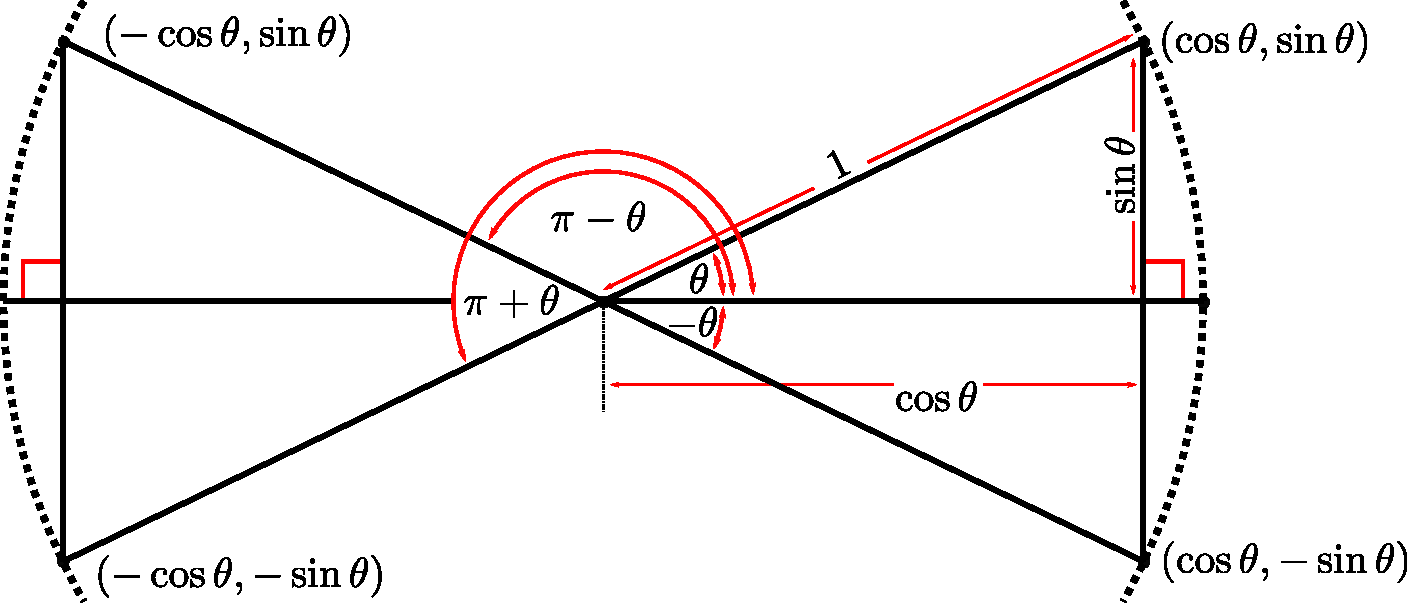
\includegraphics[height=55mm]{trig_defn5}
\end{center}
This implies that
\begin{align*}
  \sin(\pi-\theta)&=\sin(\theta) & \cos(\pi-\theta) &= -\cos(\theta) \\
  \sin(\pi+\theta)&=-\sin(\theta) & \cos(\pi+\theta) &=-\cos(\theta)
\end{align*}
From which we can get the rules for the other four trigonometric functions.


\subsection{Identities --- Adding Angles}
We wish to explain the origins of the identity
\begin{align*}
  \sin(\alpha+\beta) &= \sin(\alpha)\cos(\beta) + \cos(\alpha)\sin(\beta).
\end{align*}
A very geometric demonstration uses the figure below and an observation about areas.
\begin{center}
 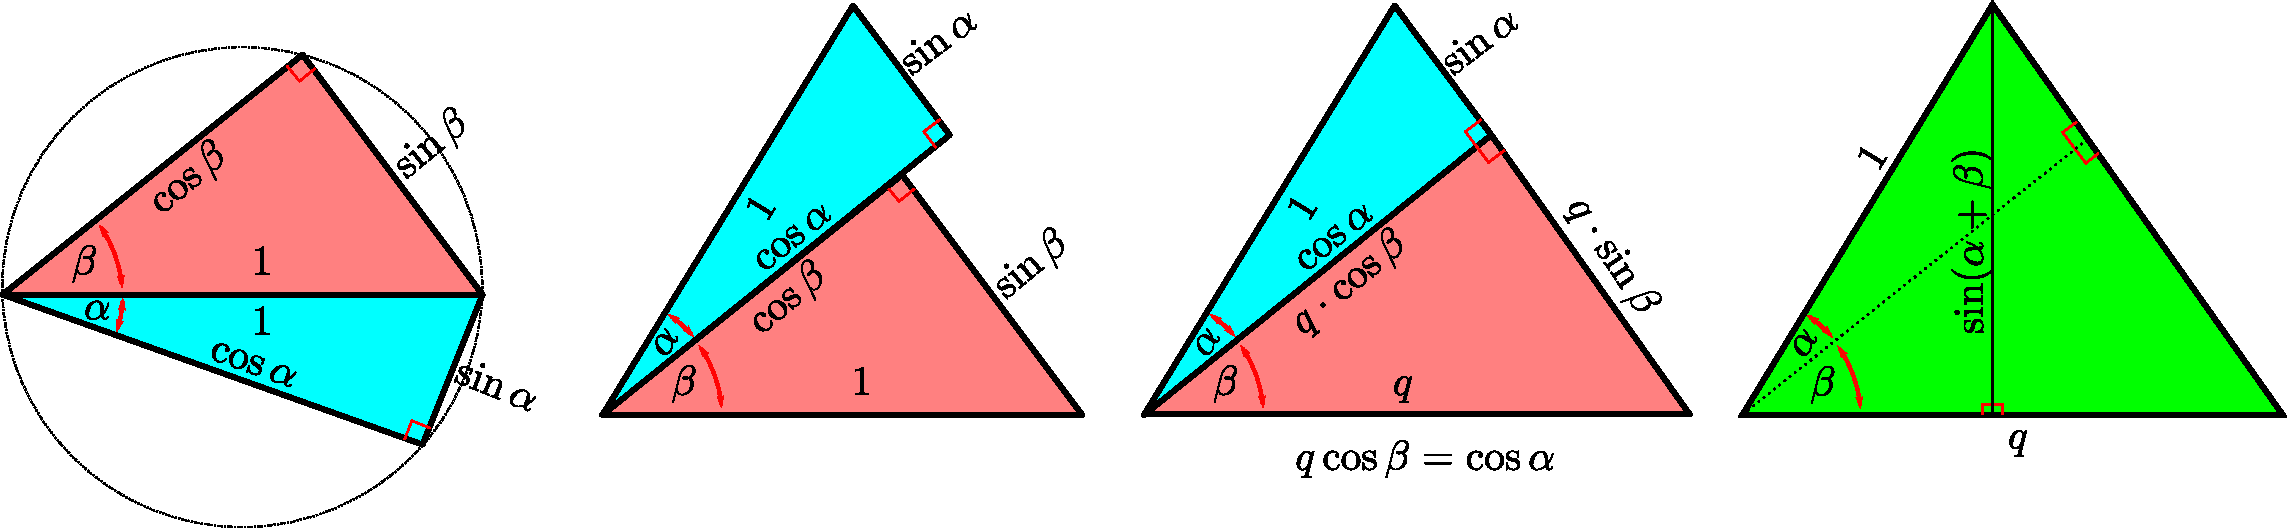
\includegraphics[width=\textwidth]{add_angles}
\end{center}
\begin{itemize}
 \item  The left-most figure shows two right-angled triangles with angles $\alpha$ and $\beta$ and both with hypotenuse length $1$.
 \item The next figure simply rearranges the triangles --- translating and rotating the lower triangle so that it lies adjacent to the top of the upper triangle.
 \item Now scale the lower triangle by a factor of $q$ so that edges opposite the angles $\alpha$ and $\beta$ are flush. This means that $q \cos \beta = \cos \alpha$. ie
\begin{align*}
  q &= \frac{\cos\alpha}{\cos\beta}
\end{align*}
  Now compute the areas of these (blue and red) triangles
  \begin{align*}
  A_\text{red} &= \frac{1}{2} q^2 \sin\beta \cos \beta \\
  A_\text{blue} &= \frac{1}{2} \sin \alpha \cos \alpha
\intertext{So twice the total area is}
  2 A_\text{total} &= \sin \alpha \cos \alpha  + q^2 \sin\beta \cos \beta
\end{align*}
\item But we can also compute the total area using the rightmost triangle:
\begin{align*}
  2 A_\text{total} &= q \sin(\alpha+\beta)
\end{align*}
\end{itemize}
Since the total area must be the same no matter how we compute it we have
\begin{align*}
q \sin(\alpha+\beta) &=  \sin \alpha \cos \alpha  + q^2 \sin\beta \cos \beta \\
  \sin(\alpha+\beta) &= \frac{1}{q} \sin \alpha \cos \alpha + q \sin\beta \cos \beta \\
  &= \frac{\cos \beta}{\cos \alpha} \sin \alpha \cos \alpha + \frac{\cos \alpha}{\cos \beta} \sin\beta \cos \beta \\
  &= \sin \alpha \cos \beta +  \cos \alpha \sin\beta
\end{align*}
as required.

We can obtain the angle addition formula for cosine by substituting $\alpha \mapsto \pi/2-\alpha$ and $\beta \mapsto -\beta$ into our sine formula:
\begin{align*}
  \sin(\alpha+\beta) &= \sin(\alpha)\cos(\beta) + \cos(\alpha)\sin(\beta) & \text{becomes}\\
  \underbrace{\sin(\pi/2-\alpha-\beta)}_{\cos(\alpha+\beta)} &= \underbrace{\sin(\pi/2-\alpha)}_{\cos(\alpha)}\cos(-\beta) + \underbrace{\cos(\pi/2-\alpha)}_{\sin(\alpha)}\sin(-\beta) \\
  \cos(\alpha+\beta) &= \cos(\alpha)\cos(\beta) - \sin(\alpha)\sin(\beta)
\end{align*}
where we have used $\sin(\pi/2-\theta)=\cos(\theta)$ and $\cos(\pi/2-\theta)=\sin(\theta)$.

It is then a small step to the formulas for the difference of angles. From the relation
\begin{align*}
  \sin(\alpha+\beta) &= \sin(\alpha)\cos(\beta) + \cos(\alpha)\sin(\beta)
\end{align*}
we can substitute $\beta \mapsto -\beta$ and so obtain
\begin{align*}
  \sin(\alpha - \beta) &= \sin(\alpha)\cos(-\beta) + \cos(\alpha)\sin(-\beta)  \\
  &= \sin(\alpha)\cos(\beta) - \cos(\alpha)\sin(\beta)
\end{align*}
The formula for cosine can be obtained in a similar manner. To summarise
\begin{align*}
  \sin(\alpha \pm \beta) &= \sin(\alpha)\cos(\beta) \pm \cos(\alpha)\sin(\beta)\\
  \cos(\alpha \pm \beta) &= \cos(\alpha)\cos(\beta) \mp \sin(\alpha)\sin(\beta)
\end{align*}

The formulas for tangent are a bit more work, but
\begin{align*}
  \tan(\alpha + \beta) &= \frac{\sin(\alpha + \beta)}{\cos(\alpha + \beta)}\\
  &= \frac{\sin(\alpha)\cos(\beta) + \cos(\alpha)\sin(\beta)}{\cos(\alpha)\cos(\beta) - \sin(\alpha)\sin(\beta) }\\
  &= \frac{\sin(\alpha)\cos(\beta) + \cos(\alpha)\sin(\beta)}{\cos(\alpha)\cos(\beta) - \sin(\alpha)\sin(\beta) }
  \cdot \frac{\sec(\alpha) \sec(\beta)}{\sec(\alpha) \sec(\beta)} \\
  &= \frac{\sin(\alpha)\sec(\alpha) + \sin(\beta)\sec(\beta)}{1 - \sin(\alpha)\sec(\alpha)\sin(\beta)\sec(\beta) } \\
  &= \frac{\tan(\alpha) + \tan(\beta)}{1 - \tan(\alpha)\tan(\beta) }
\intertext{and similarly we get}
  \tan(\alpha - \beta) &=  \frac{\tan(\alpha) - \tan(\beta)}{1 + \tan(\alpha)\tan(\beta) }
\end{align*}

\subsection{Identities --- Double-angle Formulas}
If we set $\beta=\alpha$ in the angle-addition formulas we get
\begin{align*}
  \sin(2\alpha) &= 2\sin(\alpha)\cos(\alpha) \\
  \cos(2\alpha) &= \cos^2(\alpha)-\sin^2(\alpha) \\
  &= 2\cos^2(\alpha)-1 & \text{since } \sin^2\theta =1-\cos^2\theta \\
  &= 1-2\sin^2(\alpha) & \text{since } \cos^2\theta =1-\sin^2\theta \\
  \tan(2\alpha) &= \frac{2\tan(\alpha)}{1-\tan^2(\alpha)} \\
  &= \frac{2}{\cot(\alpha)-\tan(\alpha)} &\text{divide top and bottom by
$\tan(\alpha)$}
\end{align*}

\subsection{Identities --- Extras}
\subsubsection{Sums to Products}
Consider the identities
\begin{align*}
\sin(\alpha+\beta) &= \sin(\alpha)\cos(\beta) + \cos(\alpha) \sin(\beta) &
\sin(\alpha-\beta) &= \sin(\alpha)\cos(\beta) - \cos(\alpha) \sin(\beta)
\end{align*}
If we add them together some terms on the right-hand side cancel:
\begin{align*}
\sin(\alpha+\beta) +  \sin(\alpha-\beta) &= 2\sin(\alpha)\cos(\beta).
\end{align*}
If we now set $u=\alpha+\beta$ and $v = \alpha-\beta$ (i.e. $\alpha=\frac{u+v}{2},
\beta=\frac{u-v}{2}$) then
\begin{align*}
\sin(u) +  \sin(v) &= 2\sin\left(\frac{u+v}{2}\right)\cos\left(\frac{u-v}{2}\right)
\end{align*}
This transforms a sum into a product. Similarly:
\begin{align*}
\sin(u) -  \sin(v) &= 2\sin\left(\frac{u - v}{2}\right)\cos\left(\frac{u + v}{2}\right)\\
\cos(u) +  \cos(v) &= 2\cos\left(\frac{u + v}{2}\right)\cos\left(\frac{u - v}{2}\right) \\
\cos(u) - \cos(v) &= -2\sin\left(\frac{u + v}{2}\right)\sin\left(\frac{u - v}{2}\right)
\end{align*}


\subsubsection{Products to Sums}
Again consider the identities
\begin{align*}
\sin(\alpha+\beta) &= \sin(\alpha)\cos(\beta) + \cos(\alpha) \sin(\beta) &
\sin(\alpha-\beta) &= \sin(\alpha)\cos(\beta) - \cos(\alpha) \sin(\beta)
\end{align*}
and add them together:
\begin{align*}
\sin(\alpha+\beta) +  \sin(\alpha-\beta) &= 2\sin(\alpha)\cos(\beta).
\end{align*}
Then rearrange:
\begin{align*}
\sin(\alpha)\cos(\beta)&= \frac{\sin(\alpha+\beta) +  \sin(\alpha-\beta)}{2}
\end{align*}

In a similar way, start with the identities
\begin{align*}
  \cos(\alpha+\beta) &= \cos(\alpha)\cos(\beta) - \sin(\alpha)\sin(\beta) &
  \cos(\alpha-\beta) &= \cos(\alpha)\cos(\beta) + \sin(\alpha)\sin(\beta)
\end{align*}
If we add these together we get
\begin{align*}
  2\cos(\alpha)\cos(\beta) &= \cos(\alpha+\beta) + \cos(\alpha-\beta)
\intertext{while taking their difference gives}
  2\sin(\alpha)\sin(\beta) &= \cos(\alpha-\beta) - \cos(\alpha+\beta)
\end{align*}
Hence
\begin{align*}
\sin(\alpha)\sin(\beta)&= \frac{\cos(\alpha-\beta) - \cos(\alpha+\beta)}{2}\\
\cos(\alpha)\cos(\beta)&= \frac{\cos(\alpha-\beta) + \cos(\alpha+\beta)}{2}
\end{align*}

\longsection{Inverse Trigonometric Functions}{Inverse trig functions}
In order to construct inverse trigonometric functions we first have to
restrict their domains so as to make them one-to-one (or injective). We do this as shown
below
\begin{center}
\renewcommand{\arraystretch}{2}
\begin{tabular}{|c|c|c|}
\hline
$\sin\theta$ & $\cos \theta $ & $\tan \theta$\\
\hline
Domain: $-\frac{\pi}{2} \leq \theta \leq \frac{\pi}{2}$&
Domain: $0 \leq \theta \leq \pi$&
Domain: $-\frac{\pi}{2} < \theta < \frac{\pi}{2}$\\
Range: $-1 \leq \sin \theta \leq 1$&
Range: $-1 \leq \cos \theta \leq 1$&
Range: all real numbers\\
\hline
 \begin{tikzpicture}
\begin{axis}[
  legend pos = north west,
  axis x line=center, axis y line=center,
  ymax=1.1,ymin=-1.1, ytick={-1,1},
  xmin=-2, xmax=2,
  xtick={-1.570796327,1.570796327},
  xticklabels={$-\frac{\pi}{2}$, $\frac{\pi}{2}$}
  ]
\addplot[blue,domain=-0.5*pi:0.5*pi,samples=100] {sin(deg(x))};
% \legend{$\sin \theta$}
\end{axis}
\end{tikzpicture}
&
\begin{tikzpicture}
\begin{axis}[
  axis x line=center, axis y line=center,
  ymax=1.1,ymin=-1.1, ytick={-1,1},
  xmin=-0.3,xmax=3.4,
  xtick={0,1.570796327,3.141592654},
  xticklabels={0,$\frac{\pi}{2}$, $\pi$}
  ]
\addplot[blue,domain=0:pi,samples=100] {cos(deg(x))};
% \legend{$\cos \theta$}
\end{axis}
\end{tikzpicture}
&
\begin{tikzpicture}
\begin{axis}[
  legend pos = north west,
  axis x line=center, axis y line=center,
  ymax=4.1,ymin=-4.1, ymajorticks=false,
  xmin=-2,xmax=2,
  xtick={-1.570796327,1.570796327},
  xticklabels={$-\pi$, $-\frac{\pi}{2}$}
  ]
\addplot[blue,domain=-0.49*pi:0.49*pi,samples=100] {tan(deg(x))};
% \legend{$\tan \theta$}

\addplot[line width=1pt,red] coordinates {(-1.570796327,4.15) (-1.570796327,-4.15)};
\addplot[line width=1pt,red] coordinates {(1.570796327,4.15) (1.570796327,-4.15)};
\end{axis}
\end{tikzpicture}\\
\hline\hline
$\arcsin x$ & $\arccos x$ & $\arctan x$\\
\hline
Domain: $-1 \leq x \leq 1$&
Domain: $-1 \leq x \leq 1$&
Domain: all real numbers\\
Range: $-\frac{\pi}{2} \leq \arcsin x \leq \frac{\pi}{2}$&
Range: $0 \leq \arccos x \leq \pi$&
Range: $-\frac{\pi}{2} < \arctan x < \frac{\pi}{2}$\\
\hline
\begin{tikzpicture}
\begin{axis}[
  legend pos = north west,
  axis x line=center, axis y line=center,
  xmax=1.1,xmin=-1.1, xtick={-1,1},
  ymin=-2, ymax=2,
  ytick={-1.570796327,1.570796327},
  yticklabels={$-\frac{\pi}{2}$, $\frac{\pi}{2}$}
  ]
\addplot[blue,domain=-1:1,samples=100] {asin(x)/180*pi};
% \legend{$\arcsin \theta$}
\end{axis}
\end{tikzpicture}
&
\begin{tikzpicture}
\begin{axis}[
  axis x line=center, axis y line=center,
  xmax=1.1,xmin=-1.1, xtick={-1,1},
  ymin=-0.3,ymax=3.4,
  ytick={0,1.570796327,3.141592654},
  yticklabels={0,$\frac{\pi}{2}$, $\pi$}
  ]
 \addplot[blue,domain=-1:1,samples=100] {acos(x)/180*pi};
% \legend{$\cos \theta$}
\end{axis}
\end{tikzpicture}
&
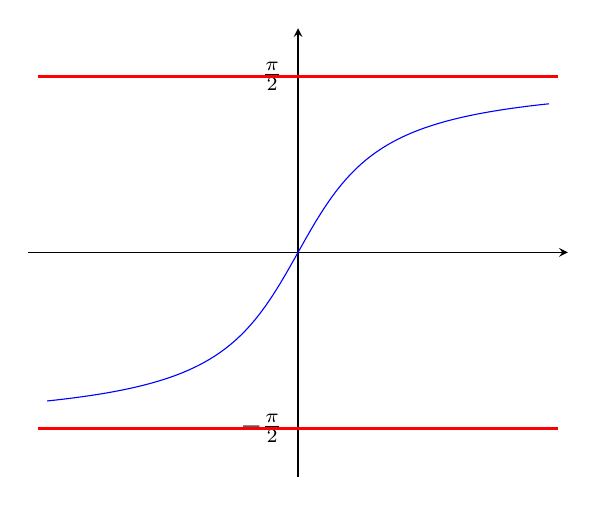
\begin{tikzpicture}
\begin{axis}[
  legend pos = north west,
  axis x line=center, axis y line=center,
  xmax=4.3,xmin=-4.3, xmajorticks=false,
  ymin=-2,ymax=2,
  ytick={-1.570796327,1.570796327},
  yticklabels={$-\frac{\pi}{2}$, $\frac{\pi}{2}$}
  ]
\addplot[blue,domain=-4:4,samples=100] {atan(x)/180*pi};
% \legend{$\tan \theta$}

\addplot[line width=1pt,red] coordinates {(4.15,-1.570796327) (-4.15,-1.570796327)};
\addplot[line width=1pt,red] coordinates {(4.15,1.570796327) (-4.15,1.570796327)};
\end{axis}
\end{tikzpicture}
\\ \hline
\end{tabular}
\renewcommand{\arraystretch}{1}
\end{center}
Since these functions are inverses of each other we have
\begin{align*}
  \arcsin(\sin \theta) &= \theta & -\frac{\pi}{2} \leq \theta \leq \frac{\pi}{2} \\
  \arccos(\cos \theta) &= \theta & 0 \leq \theta \leq \pi \\
  \arctan(\tan \theta) &= \theta & -\frac{\pi}{2} \leq \theta \leq \frac{\pi}{2}
\end{align*}
and also
\begin{align*}
  \sin(\arcsin x) &= x & -1 \leq x \leq 1 \\
  \cos(\arccos x) &= x & -1 \leq x \leq 1 \\
  \tan(\arctan x) &= x & \text{any real $x$}
\end{align*}
We can read other combinations of trig functions and their inverses, like, for
example, $\cos(\arcsin x)$, off of triangles like
\begin{efig}
\begin{center}
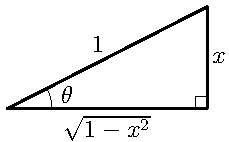
\includegraphics{../figs_differentiation/triangleAsin}
\end{center}
\end{efig}
We have chosen the hypotenuse and opposite sides of the triangle
to be of length 1 and $x$, respectively, so that
$\sin(\theta)=x$. That is, $\theta =  \arcsin x$. We can then
read off of the triangle that
\begin{align*}
  \cos(\arcsin x) &= \cos(\theta) = \sqrt{1-x^2}
\end{align*}
We can reach the same conclusion using trig identities, as
follows.
\begin{itemize}
\item Write $\arcsin x=\theta$. We know that $\sin(\theta)=x$ and we wish to
compute $\cos(\theta)$. So we just need to express $\cos(\theta)$ in terms of
$\sin(\theta)$.

 \item To do this we make use of one of the Pythagorean identities
  \begin{align*}
  \sin^2\theta + \cos^2\theta &=1\\
  \cos\theta &= \pm \sqrt{1-\sin^2\theta}
\end{align*}
\item Thus
\begin{align*}
  \cos(\arcsin x) = \cos\theta = \pm\sqrt{1-\sin^2\theta}
\end{align*}

 \item To determine which branch we should use we need to consider the domain
and range of $\arcsin x$:
\begin{align*}
  \text{Domain: } -1 \leq x \leq 1 && \text{Range: } -\frac{\pi}{2} \leq \arcsin x \leq \frac{\pi}{2}
\end{align*}
  Thus we are applying cosine to an angle that always lies between $-\frac{\pi}{2}$ and $\frac{\pi}{2}$. Cosine is non-negative on this range. Hence we should take the positive branch and
\begin{align*}
  \cos(\arcsin x) &= \sqrt{1-\sin^2\theta}= \sqrt{1-\sin^2(\arcsin x)} \\
  &= \sqrt{1-x^2}
\end{align*}
\end{itemize}
In a very similar way we can simplify $\tan(\arccos x)$.
\begin{itemize}
\item Write $\arccos x=\theta$, and then
\begin{align*}
  \tan( \arccos x) &= \tan \theta = \frac{\sin\theta}{\cos \theta}
\end{align*}
\item Now the denominator is easy since $\cos \theta = \cos \arccos x = x$.
\item The numerator is almost the same as the previous computation.
\begin{align*}
  \sin\theta &= \pm \sqrt{1-\cos^2\theta} \\
  &= \pm \sqrt{1-x^2}
\end{align*}
 \item To determine which branch we again consider domains and
and ranges:
\begin{align*}
  \text{Domain: } -1 \leq x \leq 1 && \text{Range: } 0 \leq \arccos
x \leq \pi
\end{align*}
  Thus we are applying sine to an angle that always lies between
$0$ and $\pi$. Sine is non-negative on this range and so we take the positive
branch.
\item Putting everything back together gives
\begin{align*}
  \tan(\arccos x) &= \frac{\sqrt{1-x^2}}{x}
\end{align*}

\end{itemize}


Completing the 9 possibilities gives:
\begin{align*}
  \sin( \arcsin x ) &= x &
  \sin( \arccos x ) &= \sqrt{1-x^2} &
  \sin( \arctan x ) &= \frac{x}{\sqrt{1+x^2}} \\
%
  \cos( \arcsin x ) &= \sqrt{1-x^2} &
  \cos( \arccos x ) &= x &
  \cos( \arctan x ) &= \frac{1}{\sqrt{1+x^2}} \\
%
  \tan( \arcsin x ) &= \frac{x}{\sqrt{1-x^2}} &
  \tan( \arccos x ) &= \frac{\sqrt{1-x^2}}{x} &
  \tan( \arctan x ) &= x
\end{align*}

% \end{comment}

\section{Geometry}
\subsection{Cosine Law or Law of Cosines}\label{app cosine law}
The cosine law says that, if a triangle has sides of length $a$, $b$ and $c$ and
the angle opposite the side of length $c$ is $\gamma$, then
\begin{align*}
  c^2 &= a^2+b^2 - 2ab\cos\gamma
\end{align*}
Observe that, when $\gamma=\tfrac{\pi}{2}$, this reduces to, (surpise!)
Pythagoras' theorem $c^2=a^2+b^2$. Let's derive the cosine law.
\begin{center}
 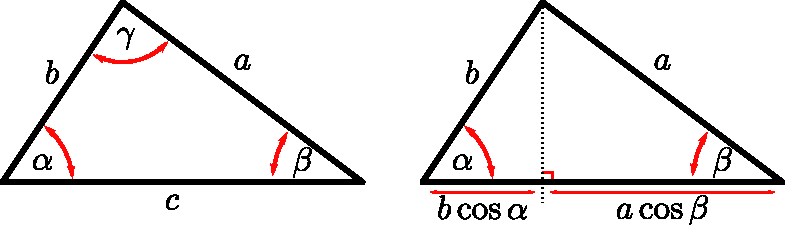
\includegraphics[height=3cm]{cosines}
\end{center}

Consider the triangle on the left. Now draw a perpendicular line from the side
of length $c$ to the opposite corner as shown. This demonstrates that
\begin{align*}
  c &= a \cos \beta + b \cos \alpha
\intertext{Multiply this by $c$ to get an expression for $c^2$:}
  c^2 &= ac \cos \beta + bc \cos \alpha
\intertext{Doing similarly for the other corners gives}
  a^2 &= ac \cos \beta + ab \cos \gamma \\
  b^2 &= bc \cos \alpha + ab \cos \gamma
\end{align*}
Now combining these:
\begin{align*}
  a^2+b^2-c^2 &=  (bc-bc) \cos \alpha + (ac-ac)\cos\beta + 2ab \cos \gamma \\
  &= 2ab\cos \gamma
\end{align*}
as required.

\subsection{Sine Law or Law of Sines}
The sine law says that, if a triangle has sides of length $a, b$ and $c$ and
the angles opposite those sides are $\alpha$, $\beta$ and $\gamma$, then
\begin{align*}
  \frac{a}{\sin \alpha} &= \frac{b}{\sin \beta} = \frac{c}{\sin \gamma}.
\end{align*}
\begin{center}
 \includegraphics[height=3cm]{sines}
\end{center}
This rule is best understood by computing the area of the triangle using the
formula $A = \frac{1}{2}ab\sin\theta$ of Appendix~\ref{app sec areas}. Doing
this three ways gives
\begin{align*}
  2A &= bc \sin \alpha \\
  2A &= ac \sin \beta \\
  2A &= ab \sin \gamma
\end{align*}
Dividing these expressions by $abc$ gives
\begin{align*}
  \frac{2A}{abc} &= \frac{\sin \alpha}{a} = \frac{\sin\beta}{b} = \frac{\sin \gamma}{c}
\end{align*}
as required.

\subsection{Where Does the Formula for the Area of a Circle Come From?}
Typically when we come across $\pi$ for the first time it is as the ratio of the
circumference of a circle to its diameter
\begin{align*}
  \pi &= \frac{C}{d} = \frac{C}{2r}
\end{align*}
Indeed this is typically the first definition we see of $\pi$.  It is easy to build an intuition that the area of the circle should be propotional to the square of its radius. For example we can draw the largest possible square inside the circle (an \emph{inscribed} square) and the smallest possible square outside the circle (a \emph{circumscribed} square):
\begin{center}
 \includegraphics[height=35mm]{archimedes0}
\end{center}
The smaller square has side-length $\sqrt{2} r$ and the longer has side-length $2r$. Hence
\begin{align*}
  2 r^2 & \leq A \leq 4r^2 & \text{ or }  2 & \leq \frac{A}{r^2} \leq 4
\end{align*}
That is, the area of the circle is between 2 and 4 times the square of the radius. What is perhaps less obvious (if we had not been told this in school) is that the constant of propotionality for area is also $\pi$:
\begin{align*}
  \pi &= \frac{A}{r^2}.
\end{align*}


We will show this using Archimedes' proof. He makes use of these inscribed and circumscribed polygons to make better and better approximations of the circle. The steps of the proof are somewhat involved and the starting point is to rewrite the area of a circle as
\begin{align*}
  A &= \frac{1}{2} C r
\end{align*}
where $C$ is (still) the circumference of the circle. This suggests that this
area is the same as that of a triangle of height $r$ and base
length $C$
\begin{align*}
  T &= \frac{1}{2} C r
\end{align*}
\begin{center}
 \includegraphics[height=3cm]{archimedes1}
\end{center}
Archimedes' proof then demonstrates that indeed this triangle and the circle have the same
area. It relies on a ``proof by contradiction'' --- showing that $T<A$ and $T>A$ cannot
be true and so the only possibility is that $A=T$.

We will first show that $T<A$ cannot happen. Construct an $n$-sided ``inscribed'' polygon
as shown below:
\begin{center}
 \includegraphics[height=4cm]{archimedes2}
\end{center}
Let $p_n$ be the inscribed polygon as shown.
\begin{center}
 \includegraphics[width=\textwidth]{archimedes3}
\end{center}
We need 4 steps.
\begin{enumerate}
 \item The area of $p_n$ is smaller than that of the circle --- this follows since we can
construct $p_n$ by cutting slices from the circle.
 \item Let $E_n$ be the difference between the area of the circle and $p_n$: $E_n = A -
A(p_n)$ (see the left of the previous figure). By the previous point we know $E_n>0$.
Now as we increase the number of sides, this difference becomes smaller. To be more
precise
  \begin{align*}
  E_{2n} & \leq \frac{1}{2} E_n.
  \end{align*}
The error $E_n$ is made up of $n$ ``lobes''. In the centre-left of the previous figure we
draw one such lobe and surround it by a rectangle of dimensions $a \times 2b$ --- we
could determine these more precisely using a little trigonometry, but it is not necessary.

This diagram shows the lobe is smaller than the rectangle of base $2b$ and height $a$
Since there are $n$ copies of the lobe, we have
\begin{align*}
  E_n & \leq n  \times 2ab & \text{rewrite as } \frac{E_n}{2} & \leq nab
\end{align*}

Now draw in the polygon $p_{2n}$ and consider the associated ``error'' $E_{2n}$. If we
focus on the two lobes shown then we see that the area of these two new lobes is equal to
that of the old lobe (shown in centre-left) minus the area of the triangle with base $2b$
and height $a$ (drawn in purple). Since there are $n$ copies of this
picture we have
\begin{align*}
  E_{2n} &= E_n - nab & \text{now use that $nab \geq  E_n/2$} \\
  & \leq E_n - \frac{E_n}{2} = \frac{E_n}{2}
\end{align*}

\item The area of $p_n$ is smaller than $T$. To see this decompose $p_n$ into $n$
isosceles triangles. Each of these has base shorter than $C/n$; the straight line is
shorter than the corresponding arc --- though strictly speaking we should prove this. The
height of each triangle is shorter than $r$. Thus
\begin{align*}
  A(p_n) &= n \times \frac{1}{2} \text{(base)}\times \text{(height)} \\
  & \leq n \times \frac{Cr}{2n} = T
\end{align*}

\item If we assume that $T<A$, then $A-T = d$ where $d$ is some positive number.
However we know from point 2 that we can make $n$ large enough so that $E_n < d$
(each time we double $n$ we halve the error). But now we have a contradiction to
step~3, since we have just shown that
\begin{align*}
  E_n = A-A(p_n) & < A-T & \text{which implies that}\\
  A(p_n) & > T.
\end{align*}
\end{enumerate}
Thus we cannot have $T<A$.

If we now assume that $T>A$ we will get a similar contradiction by a similar
construction. Now we use regular $n$-sided \emph{circumscribed} polygons, $P_n$.
\begin{center}
 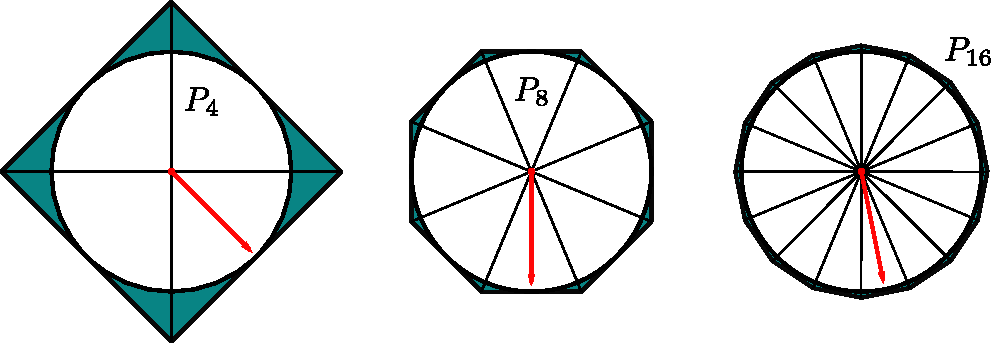
\includegraphics[height=35mm]{archimedes4}
\end{center}
The proof can be broken into 4 similar steps.
\begin{center}
 \includegraphics[width=\textwidth]{archimedes5}
\end{center}
\begin{enumerate}
 \item The area of $P_n$ is greater than that of the circle --- this follows since we
can construct the circle by trimming the polygon $P_n$.

 \item Let $E_n$ be the difference between the area of the polygon and the circle: $E_n =
A(P_n)-A$ (see the left of the previous figure). By the previous point we know $E_n>0$.
Now as we increase the number of sides, this difference becomes smaller. To be more
precise we will show
  \begin{align*}
  E_{2n} & \leq \frac{1}{2} E_n.
  \end{align*}
The error $E_n$ is made up of $n$ ``lobes''. In the centre-left of the previous figure we
draw one such lobe. Let $L_n$ denote the area of one of these lobes, so $E_n = nL_n$.  In
the centre of the previous figure we have labelled this lobe carefully and also shown how
it changes when we create the polygon $P_{2n}$. In particular, the original lobe is
bounded by the straight lines $\vec{ad}, \vec{af}$ and the arc $\widehat{fbd}$. We create
$P_{2n}$ from $P_n$ by cutting away the corner triangle $\triangle aec$. Accordingly the
lines $\vec{ec}$ and $\vec{ba}$ are orthogonal and the segments $|bc|=|cd|$.

By the construction of $P_{2n}$ from $P_n$, we have
\begin{align*}
  2L_{2n} &= L_n - A( \triangle aec) & \text{or equivalently }
  L_{2n} &= \frac{1}{2} L_n - A( \triangle abc)
\end{align*}
And additionally
\begin{align*}
  L_{2n} & \leq A( \triangle bcd)
\end{align*}

Now consider the triangle $\triangle abd$ (centre-right of the previous figure) and the
two triangles within it $\triangle abc$ and $\triangle bcd$. We know that $\vec{ab}$ and
$\vec{cb}$ form a right-angle. Consequently $\vec{ac}$ is the hypotenuse of a right-angled
triangle, so $|ac|>|bc| = |cd|$. So now, the triangles $\triangle abc$ and $\triangle bcd$
have the same heights, but the base of $\vec{ac}$ is longer than $\vec{cd}$. Hence the
area of $\triangle abc$ is strictly larger than that of $\triangle bcd$.

Thus we have
\begin{align*}
  L_{2n} & \leq A(\triangle bcd) < A(\triangle abc)
\end{align*}
But now we can write
\begin{align*}
  L_{2n} &= \frac{1}{2} L_n - A( \triangle abc) < \frac{1}{2} L_n - L_{2n}  &
\text{rearrange}\\
  2L_{2n} &< \frac{1}{2} L_n & \text{there are $n$ such lobes, so } \\
  2n L_{2n} &< \frac{n}{2} L_n & \text{since $E_n = n L_n$, we have}\\
  E_{2n} & < \frac{1}{2} E_n & \text{which is what we wanted to show.}
\end{align*}


\item The area of $P_n$ is greater than $T$. To see this decompose $P_n$ into $n$
isosceles triangles. The height of each triangle is $r$, while the base of each is longer
than $C/n$ (this is a subtle point and its proof is equivalent to showing that $\tan
\theta > \theta$). Thus
\begin{align*}
  A(P_n) &= n \times \frac{1}{2} \text{(base)}\times \text{(height)} \\
  & \geq n \times \frac{Cr}{2n} = T
\end{align*}

\item If we assume that $T>A$, then $T-A = d$ where $d$ is some positive number.
However we know from point 2 that we can make $n$ large enough so that $E_n < d$ (each
time we double $n$ we halve the error). But now we have a contradiction since we have just
shown that
\begin{align*}
  E_n = A(P_n) - A & < T-A & \text{which implies that}\\
  A(p_n) & > T.
\end{align*}
\end{enumerate}
Thus we cannot have $T>A$. The only possibility that remains is that $T=A$.


\subsection{Where Do These Volume Formulas Come From?}\label{apendix volume}
We can establish the volumes of cones and spheres from the formula for the volume of a
cylinder and a little work with limits and some careful summations. We first need a few
facts.
\begin{itemize}
 \item Every square number can be written as a sum of consecutive odd numbers. More
precisely
  \begin{align*}
  n^2 &= 1 + 3 + \dots (2n-1)
\end{align*}
 \item The sum of the first $n$ positive integers is $\frac{1}{2} n(n+1)$. That is
\begin{align*}
  1 + 2 +3 +\dots +n &= \frac{1}{2}n(n+1)
\end{align*}
 \item The sum of the squares of the first $n$ positive integers is $\frac{1}{6}
n(n+1)(2n+1)$.
\begin{align*}
  1^2 + 2^2 +3^2 +\dots + n^2 &= \frac{1}{6}n(n+1)(2n+1)
\end{align*}
\end{itemize}
We will not give completely rigorous proofs of the above identities (since we are not
going to assume that the reader knows mathematical induction), rather we will explain
them using pictorial arguments. The first two of these we can explain by some quite simple
pictures:
\begin{center}
 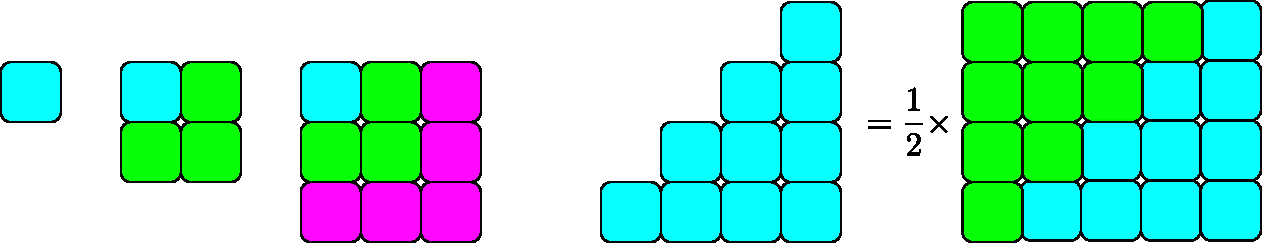
\includegraphics[width=\textwidth]{sums1}
\end{center}
We see that we can decompose any square of unit-squares into a sequence of strips, each
of which consists of an odd number of unit-squares. This is really just from the fact that
\begin{align*}
  n^2 - (n-1)^2 &= 2n-1
\end{align*}
Similarly, we can represent the sum of the first $n$ integers as a triangle of unit
squares as shown. If we make a second copy of that triangle and arrange it as shown, it
gives a rectangle of dimensions $n$ by $n+1$. Hence the rectangle, being exactly twice the
size of the original triangle, contains $n(n+1)$ unit squares.

The explanation of the last formula takes a little more work and a carefully
constructed picture:
\begin{center}
 \includegraphics[width=\textwidth]{sums2}
\end{center}
Let us break these pictures down step by step
\begin{itemize}
 \item Leftmost represents the sum of the squares of the first $n$ integers.
 \item Centre --- We recall from above that each square number can be written as a sum of
consecutive odd numbers, which have been represented as coloured bands of unit-squares.
 \item Make three copies of the sum and arrange them carefully as shown. The first and
third copies are obvious, but the central copy is rearranged considerably; all
bands of the same colour have the same length and have been arranged into
rectangles as shown.

Putting everything from the three copies together creates a rectangle of dimensions
$(2n+1)\times(1+2+3+\dots+n)$.
\end{itemize}
We know (from above) that $1+2+3+\dots+n = \frac{1}{2} n(n+1)$ and so
\begin{align*}
  (1^2+2^2+\dots+n^2 ) &= \frac{1}{3} \times \frac{1}{2} n(n+1)(2n+1)
\end{align*}
as required.

Now we can start to look at volumes. Let us start with the volume of a cone; consider the
figure below. We bound the volume of the cone above and below by stacks of cylinders. The
cross-sections of the cylinders and cone are also shown.
\begin{center}
 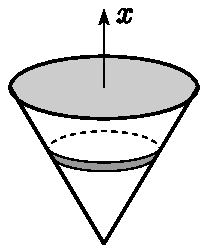
\includegraphics[width=0.8\textwidth]{cone}
\end{center}
To obtain the bounds we will construct two stacks of $n$ cylinders, $C_1,C_2,\dots,C_n$.
Each cylinder has height $h/n$ and radius that varies with height. In particular, we
define cylinder $C_k$ to have height $h/n$ and radius $k \times r/n$. This radius was
determined using similar triangles so that cylinder $C_n$ has radius $r$. Now cylinder
$C_k$ has volume
\begin{align*}
  V_k &= \pi \times \text{radius}^2 \times \text{height}
  = \pi \left( \frac{kr}{n} \right)^2 \cdot \frac{h}{n}\\
  &= \frac{\pi r^2h}{n^3} k^2
\end{align*}

We obtain an upper bound by stacking cylinders $C_1,C_2,\dots,C_n$ as shown. This object
has volume
\begin{align*}
  V &= V_1 + V_2 + \dots V_n \\
  &= \frac{\pi r^2h}{n^3} \left(1^2 + 2^2 + 3^2 + \dots + n^2 \right) \\
  &= \frac{\pi r^2h}{n^3} \cdot \frac{n(n+1)(2n+1)}{6}
\end{align*}
A similar lower bound is obtained by stacking cylinders $C_1,\dots,C_{n-1}$ which gives a
volume of
\begin{align*}
  V &= V_1 + V_2 + \dots V_{n-1} \\
  &= \frac{\pi r^2h}{n^3} \left(1^2 + 2^2 + 3^2 + \dots + (n-1)^2 \right) \\
  &= \frac{\pi r^2h}{n^3} \cdot \frac{(n-1)(n)(2n-1)}{6}
\end{align*}
Thus the true volume of the cylinder is bounded between
\begin{align*}
  \frac{\pi r^2h}{n^3} \cdot \frac{(n-1)(n)(2n-1)}{6}
  & \leq \text{correct volume}
  \leq \frac{\pi r^2h}{n^3} \cdot \frac{n(n+1)(2n+1)}{6}
\end{align*}
We can now take the limit as the number of cylinders, $n$, goes to infinity. The upper
bound becomes
\begin{align*}
  \lim_{n \to \infty} \frac{\pi r^2h}{n^3} \frac{n(n+1)(2n+1)}{6}
  &= \frac{\pi r^2h}{6} \lim_{n\to\infty} \frac{n(n+1)(2n+1)}{n^3} \\
  &= \frac{\pi r^2h}{6} \lim_{n\to\infty} \frac{(1+1/n)(2+1/n)}{1} \\
  &= \frac{\pi r^2h}{6} \times 2 \\
  &= \frac{\pi r^2h}{3}
\end{align*}
The other limit is identical, so by the squeeze theorem we have
\begin{align*}
  \text{Volume of cone } &= \frac{1}{3} \pi r^2h
\end{align*}

Now the sphere --- though we will do the analysis for a hemisphere of radius $R$. Again
we bound the volume above and below by stacks of cylinders. The cross-sections of the
cylinders and cone are also shown.
\begin{center}
 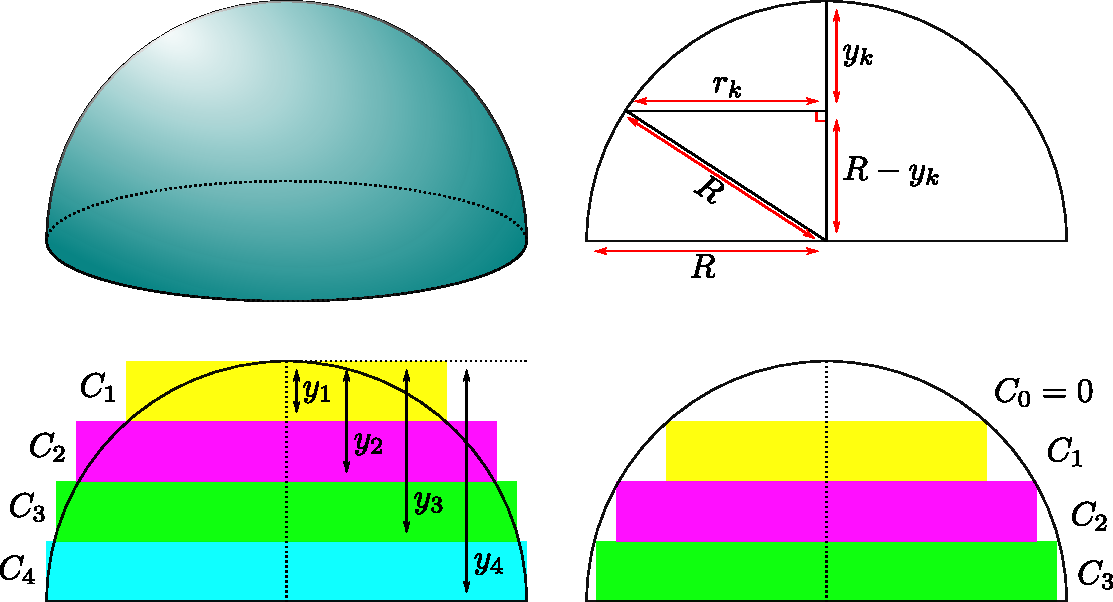
\includegraphics[width=0.8\textwidth]{sphere}
\end{center}
To obtain the bounds we will construct two stacks of $n$ cylinders, $C_1,C_2,\dots,C_n$.
Each cylinder has height $R/n$ and radius that varies with its position in the
stack. To describe the position, define
\begin{align*}
  y_k &= k \times \frac{R}{n}
\end{align*}
That is, $y_k$, is $k$ steps of distance $\frac{R}{n}$ from the top of the
hemisphere. Then we set the $k^\mathrm{th}$ cylinder, $C_k$ to have height $R/n$
and radius $r_k$ given by
\begin{align*}
  r_k^2 &= R^2 - (R-y_k)^2 = R^2 - R^2(1-k/n)^2 \\
  &= R^2( 2k/n - k^2/n^2)
\end{align*}
as shown in the top-right and bottom-left illustrations. The volume of $C_k$ is then
\begin{align*}
  V_k &= \pi \times \text{radius}^2 \times \text{height}
  = \pi \times R^2 \left(2k/n - k^2/n^2  \right) \times \frac{R}{n}\\
  &=  \pi R^3 \cdot \left( \frac{2k}{n^2}  - \frac{k^2}{n^3} \right)
\end{align*}

We obtain an upper bound by stacking cylinders $C_1,C_2,\dots,C_n$ as shown. This object
has volume
\begin{align*}
  V &= V_1 + V_2 + \dots V_n \\
  &=
\pi R^3 \cdot \left( \frac{2}{n^2}\left(1 + 2 + 3 + \dots + n \right)
- \frac{1}{n^3}\left(1^2 + 2^2 + 3^2 + \dots + n^2 \right) \right)
\end{align*}
Now recall from above that
\begin{align*}
  1 + 2 + 3 + \dots +n &= \frac{1}{2} n(n+1) &
  1^2 + 2^2 + 3^2 + \dots +n^2 &= \frac{1}{6} n(n+1)(2n+1)
\end{align*}
so
\begin{align*}
  V &= \pi R^3 \cdot \left( \frac{n(n+1)}{n^2}
- \frac{n(n+1)(2n+1)}{6n^3} \right)
\end{align*}

Again, a lower bound is obtained by stacking cylinders $C_1,\dots,C_{n-1}$ and a similar
analysis gives
\begin{align*}
  V &= \pi R^3 \cdot \left( \frac{n(n-1)}{(n-1)^2}
- \frac{n(n-1)(2n-1)}{6(n-1)^3} \right)
\end{align*}

Thus the true volume of the hemisphere is bounded between
\begin{align*}
  \pi R^3 \cdot \left( \frac{n(n+1)}{n^2}
- \frac{n(n+1)(2n+1)}{6n^3} \right)
  & \leq \text{correct volume}
  \leq \pi R^3 \cdot \left( \frac{n(n+1)}{n^2}
- \frac{n(n+1)(2n+1)}{6n^3} \right)
\end{align*}
We can now take the limit as the number of cylinders, $n$, goes to infinity. The upper
bound becomes
\begin{align*}
  \lim_{n \to \infty} \pi R^3 \cdot \left( \frac{n(n+1)}{n^2}
- \frac{n(n+1)(2n+1)}{6n^3} \right)
  &= \pi R^3 \left( \lim_{n\to\infty} \frac{n(n+1)}{n^2} -
\frac{n(n+1)(2n+1)}{6n^3}
\right)\\
  &= \pi R^3 \left( 1 - \frac{2}{6} \right) = \frac{2}{3} \pi R^3.
\end{align*}
The other limit is identical, so by the squeeze theorem we have
\begin{align*}
  \text{Volume of hemisphere } &= \frac{2}{3} \pi R^3 & \text{ and so}\\
  \text{Volume of sphere } &= \frac{4}{3} \pi R^3
\end{align*}

\end{comment}
